\documentclass[a4paper,11pt]{report}
%
%--------------------   start of the 'preamble'
%
\usepackage{amssymb,amstext,amsmath}
\usepackage{pdfpages} 
\usepackage[latin1]{inputenc}
\usepackage{fullpage}
\usepackage{caption}
\usepackage{color}
\usepackage{epstopdf}
\usepackage{graphicx}
\usepackage{todonotes}
\usepackage{graphics}
\usepackage[pdftex]{epsfig}
\usepackage{lscape}
\usepackage{rotating}
\usepackage{enumerate}
\usepackage{multirow}
\usepackage{array}


%
%%    homebrew commands -- to save typing
\newcommand\etc{\textsl{etc}}
\newcommand\eg{\textsl{eg.}\ }
\newcommand\etal{\textsl{et al.}}
\newcommand\Quote[1]{\lq\textsl{#1}\rq}
\newcommand\fr[2]{{\textstyle\frac{#1}{#2}}}
\newcommand\miktex{\textsl{MikTeX}}
\newcommand\comp{\textsl{The Companion}}
\newcommand\nss{\textsl{Not so Short}}
\newcommand{\HRule}{\rule{\linewidth}{0.5mm}}
\newcommand \cc[1]{\textcolor{red}{\textsl{-CESAR-}}{\textcolor{red}{#1}}} %comments from cesar
\newcommand \cm[1]{\textcolor{blue}{\textsl{-MACIEJ-}}{\textcolor{blue}{#1}}}


\newcommand{\tab}{\hspace*{2em}}

%=============== Temporary solutions to naming problem ======================

% full names
% if you need space after the command,use "\" i.e. "
% \HighPriority is" ==>> will change into "High Priorityis"
% \HighPriority\ is" ==>> will change into "High Priority is"
\newcommand \HighPriority[0]{High Priority}
\newcommand \StandardPriority[0]{Standard Priority}
\newcommand \GranularityWindow[0]{Granularity Window}
\newcommand \ControlMessage[0]{Control Message} %White Rabbit Information Block


% abreviations
\newcommand \HP[0]{HP}
\newcommand \SP[0]{SP}
\newcommand \GW[0]{GW}
\newcommand \CM[0]{CM} % WRIB

%=============================================================================

%comments from cesar
%
\graphicspath{{fig/}}
%\graphicspath{{.}}
%---------------------   end of the 'preamble'
%

%TO REMOVE THE WRITTEN CHAPTER FROM THE CHAPTER
\makeatletter
\renewcommand{\@makechapterhead}[1]{%
\vspace*{0pt}%
{\setlength{\parindent}{0pt} \raggedright \normalfont
\bfseries\huge\thechapter.\ #1
\par\nobreak\vspace{40 pt}}}
\makeatother


\graphicspath{ {../../../../figures/} }

\begin{document}
%-----------------------------------------------------------
\title{Robustness and Determinism in White Rabbit}
\author{Cesar Prado GSI}
\author{Maciej Lipinski CERN}
\date
\maketitle

\begin{titlepage}
 
\begin{center}

% Upper part of the page
%\includegraphics[scale=0.50]{fig/white_rabbit.jpg}\\[1cm]
%\includegraphics[height=80mm]{white_rabbit.ps}\\[1cm]
\includegraphics[height=70mm]{logo/WRlogo.ps}\\[1cm]

% Title
\HRule \\[0.4cm]
{ \huge \bfseries White Rabbit and Robustness \\ [0.8cm]
  \Large Draft for Comments}\\[0.4cm]
\HRule \\[1.0cm]
 
\textsc{\normalsize  GSI, Helmholtzzentrum fur Schwerionenforschung GmbH}
\newline
\textsc{\normalsize  CERN, Organisation Europeenne pour la Recherche Nucleaire}
\\[0.5cm]

% Author and supervisor
%\begin{minipage}{0.4\textwidth}
\begin{flushright} \large
Cesar Prados, Maciej Lipinski
\end{flushright}
%\end{minipage}
 
\vfill
 
% Bottom of the page
\begin{flushright}
{\large \today}
\end{flushright}
 
\end{center}
 
\end{titlepage}


%-----------------------------------------------------------
%\begin{abstract}\centering
%\end{abstract}
%-----------------------------------------------------------
\tableofcontents
%-----------------------------------------------------------
%\centering
\paragraph*{Revision History Table}

\begin{center}
\begin{tabular}{|p{1.5 cm}|p{2 cm}|p{1.5 cm}|p{6 cm}|} \hline

\textbf{Version} & \textbf{Date} & \textbf{Authors} & \textbf{Description} \\
\hline
0.1 & 1/09/2010 & C.P & first draft \\ \hline
0.2 & 3/02/2011 & M.L. & made a lot of mess \\ \hline
0.3 & 23/02/2011 & M.L. & Change of doc's strucutre based on feedback (yet more
mess...)\\ \hline
0.4 & 15/03/2011 & C.P \& M.L. & Minor, and less minor changes to make it look
 better and be more readable. \\ \hline
\end{tabular}
\end{center}



%\centering
\paragraph*{List of Acronyms}

\vspace{3 cm}

\normalsize
\begin{flushleft}
	\begin{tabular}{lcl} 
		WR & : & White Rabbit \\ 
		PTP & : & Precision Time Protocol \\
		WRPTP & : & White Rabbit extension PTP \\
		\HP & : & High Priority. Used to indicate special WR Ethernet
			Frames\\
		\SP & : & Standard Priority. Used to indicate special WR
			  Ethernet Frames\\
		&& \\
		WRN & : & White Rabbit Node \\
		WRS & : & White Rabbit Switch \\
		WRCM & : & White Rabbit Clock Master Node \\
		WRMM & : & White Rabbit Management Master Node \\
		WRDM & : & White Rabbit Data Master Node \\
		&&\\
		&&\\
		SNMP & : & Simple Network Management Protocol \\
		FEC & : & Forward Error Correction\\
		PFC & : & Priority Flow Control \\

%	     \cc{ } & : & Comment by Cesar \\
%	     \cm{ } & : & Comment by Maciej \\

	\end{tabular}
\end{flushleft}

A few of the terms (names) used in this document are a matter of discussion.
The currently used terms do not seem appropriate, they are sometimes
confusiong. The names are listed below. They are prone to be changed. A reader
is kindly asked to indicate a better name, if he/she have something in mind.

\begin{itemize}
  \item \HighPriority (\HP),
  \item \StandardPriority (\SP),
  \item \GranularityWindow (\GW),
  \item \ControlMessage (\CM).
\end{itemize}

\newpage


\chapter{Introduction}
\label{introduction}

\section{What is White Rabbit?} 

White Rabbit is intended to be the next-generation deterministic network based
on synchronous Ethernet, allowing for low-latency deterministic packet routing
and transparent, high precision timing transmission. The network consists of
White Rabbit Nodes, White Rabbit Switches and supports integration of nodes
and/or switches that are not White Rabbit, however with restrictions.


The resilience and robustness is one of the key features of any
fieldbus, specially, in safety Ethernet-based fieldbuses for critical systems
like White Rabbit. The reliability of the WR falls on the deterministic delivery
of Ethernet frames through a switching network and the synchronization of the
network devices. In order to provide a service with low error, it is necessary
to propose methods and techniques to overcome problems caused by the
imperfection of the physical medium, dropped packets in WR switches and
breakdowns of the network devices.


A White Rabbit Network, consisting of White Rabbit Switches (WRS) connected
by fibre or copper, is meant to transport information between White Rabbit
Nodes (WRN). In this document three types of information transported over White
Rabbit Network are distinguished:

\begin{itemize}
  \item  Timing Information - includes frequency and Coordinated Universal
  Time (UTC), it is sent from Timing Master to White Rabbit Switches and Nodes.
  \item  Control Data - includes \ControlMessage s (\CM), it is broadcast from
Data Master to  White Rabbit Nodes. 
  \item  Standard Data - all other Ethernet traffic sent between nodes and
  switches.
\end{itemize}
Timing Information and Control Data are considered to be critical. 
The types of information are closely related to their source. A Timing Master is
a White Rabbit Switch or Node which is connected to GPS receiver. A Data Master
is a White Rabbit Node which is responsible for \ControlMessage\   distribution.


The main component of White Rabbit Network is a White Rabbit Switch.
It is a Layer~2 network bridge which supports Synchronous Ethernet
(SyncE) \cite{SynchE} and implements White Rabbit Protocol (WRPTP) \cite{WRPTP}
which is an extension of PTP standard (IEEE1588 \cite{IEEE1588}). WRPTP, along
with SyncE, enables to distribute common notion of time and frequency over the
entire White Rabbit Network with sub-nanosecond precision. 

\section{WR Network Requirements} 

The requirements for the WR have been defined by GSI and CERN, since the
Control Sytems of their accelerator are going to be based on WR. A Control
System for accelerator facility requires high reliability, high precision and
determinism. 

Unreliability is translated into the number of \ControlMessage s not delivered
to one or more designated nodes within one year. 

In terms of reliability, it is expected to lose along the way from WR Data
Master to receiving WR Nodes only one \ControlMessage\ per year. 

Determinism in this chapter is understood as delivery of \ControlMessage\ to all
designated nodes within the required time regardless of the node's location in
the network. If the \ControlMessage\ delivery time is exceeded, the message is
considered undelivered (lost).

At GSI, White Rabbit is foreseen to control new FAIR accelerator complex. The
requirements for the new FAIR machines \cite{FAIRtiming} state that the Control
Message should be delivered from Data Master Node to all receiving devices
(Nodes) within 100$\mu s$ given the maximum distance between Data Master and a
Node of 2km \cite{FAIRtimingSystem}.

At CERN, the required time to delivered the message is 1ms but the distance 
between Data Master and a Node is substantially larger (max of 10km)
\cite{CERNtiming}.

Knowing how often a \ControlMessage\ is sent (every 100$\mu s$ at GSI and 
1000$\mu s$ at CERN), we can calculate the maximum acceptable failure rate
of WR Network ($\lambda_{WRN_{max}}$)

\begin{equation}
 \label{eq:failureProbability}
	\lambda_{WRN_{max}} = \frac{number\_of\_\ControlMessage
s\_lost\_per\_year}{number\_of\_\ControlMessage s\_sent\_per\_year}
\end{equation}


The requirements concerning \ControlMessage\ size differ between FAIR and CERN
as well. While in GSI facility a \ControlMessage\ of 1500 bytes (maximum
Ethernet Frame payload) is more than sufficient, for CERN facility it is an
acceptable value, but the expectations are higher, e.g.: 4800bytes (see
Appendix~\ref{appB}). Table~\ref{tab:requirements} summarizes the GSI's and
CERN's requirements.

\begin{table}[ht]
\caption{GSI's and CERN's requirements summary.} 
\centering
	\begin{tabular}{| c | c | c |}          \hline
\textbf{Requirement name}& \multicolumn{2}{|c|}{\textbf{Value(s)}}  \\
                         & GSI              & CERN          \\ \hline
\GranularityWindow       & 100$\mu s$       & 1000$\mu s$   \\ \hline
max Failure rate ($\lambda_{WRN_{max}}$) & $3.170979198*10^{-12}$ &
$3.170979198*10^{-11}$  \\ \hline
%min Reliability ($R_{WRN}$)& 0.999 999 999 997
% & 0.999 999 999 968\\ \hline
Maximum Link Length      & 2km              & 10km          \\ \hline
\ControlMessage Size     & 300-1500 bytes   & 1200 - 5000 bytes     \\ \hline
Synchronization accuracy & probably 8ns   & most nodes 1$\mu s$ \\
                         &                & few nodes  ~2ns \\
\hline

\end{tabular}
\label{tab:requirements}
\end{table}

\section{The Goals of This Document} 

This document introduces methods and techniques which increase 
reliability, robustness and determinism of White Rabbit Network so that the
requirements listed in the previous chapter are met. It also introduces
techniques to guard the safety of the network, monitor and 
diagnose. However, the presented solutions are considered optional. Their usage
should be considered on individual bases and according to actual needs of 
a particular use case.



Determinism, as understood in this document, can be achieved by a precise
knowledge of maximum delays introduced by each component of the network and 
optimisation of the delay to meet the requirements. 

\textbf{Chapter 2} discusses determinism of White Rabbit Network. In particular
it focuses on the \ControlMessage\ maximum delivery time from the Data Master
to WR Nodes. 

Unreliability of the system is caused by physical imperfection of network's
components. In particular, by data corruption on the physical links and failure
of network components. Reliability of data distribution in a network can be
increased by redundancy of data (special encoding) and components
(switches, links). In terms of redundancy, two types of information
distributed over White Rabbit Network are considered separately: Timing
Information and Data (Control and Standard). 

Timing Information is conveyed from a Timing Master to all nodes. Data is
sent from any node (Data Master, in case of Control Data) to one or many nodes.
Timing Information and Data are distributed along so called Paths. A Path is
understood as the cables and switches by which information traverse from the
sender to the receiver of the information. Consequently, there are two types of
paths:
\begin{itemize}
  \item Clock Path - path from Timing Master to the nodes.
  \item Data Path - path from sending node to receiving node(s).
\end{itemize}
A layout of all possible Paths in a network is called topology. Therefore we
define in White Rabbit Network:

\begin{itemize}
  \item Clock Path Topology - Layout of all possible Clock Paths in the
network.
  \item Data Path Topology - Layout of all possible Data Paths in the
network.
\end{itemize}

One of the unique features of White Rabbit Network is a precise synchronization
and syntonization of all the White Rabbit network components. Failure to deliver
this information to any White Rabbit component, or deterioration of its quality
(instability) might have sever consequences and render the network unreliable.
\textbf{Chapter 3} describes how the quality of Timing Information is
guarded, its reliability increased by introducing redundancy of Clock Path and
its stability ensured during switchover between redundant Clock Paths.

\textbf{Chapter 4} describes techniques to achieved required reliability of
Control Data delivery and substantially increase reliability of Standard Data.
This is done by introducing redundancy of network components (topology) and
redundancy of data (Forward Error Correction, EFC). Since, congestion of network
traffic is undesired and dangerous for reliable message delivery, this chapter
deals with flow control and congestion problems as well. 

\textbf{Chapter 5} focuses on techniques which allows for WR Network
monitoring as well as fast and efficient diagnostics of the network.


\chapter{Determinism} 
\label{jitterDeterminismNetworkDimention}

An Ethernet frames sent by various sources (e.g.: WR Node) will reach their
destinations with different delays. A packet's delay varies with:
\begin{itemize}
  \item the source's position in the network,
  \item the numbers of hops along the path,
  \item load of traffic ,
  \item Class of Service, priority.
\end{itemize}
This variation in delay is known as jitter. Determinism of packets' delivery in
Ethernet network is understood in this document as predictability of its delay.
A deterministic network is the one in which the delay of packet's delivery from
the source to the receiver is guaranteed to be within a set time. This time is
called \GranularityWindow (\GW). 

Carefully configured and properly used White Rabbit Network offers
deterministic Ethernet Frame delivery for routed unicast and broadcast traffic
\footnote{It is true, if the \HP\ Bypass described in
Chapter~\ref{chapter:HPbypass} is not enabled.}
(Appendix~\ref{appH} details estimation of Ethernet Frame delivery delay). This
is possible thanks to the implementation of Class of Service (CoS) and the fact
that the delay introduced by the switch can be verified by analysis of publicly
available source code. By routed traffic, we understand store-and-forward
traffic whose destination is determined by Routing Table Unit (RTU) and which is
stored and forwarded using Switching Core (Swcore). Figure~\ref{fig:swRouting}
gives an overview of the routing mechanism in WR Switch, details of WR Switch
routing implementation are available in the
presentation \cite{HWpresentation}.




In White Rabbit Network the requirements regarding determinism are
straightforward: \ControlMessage\ (which is transported by a number of Ethernet
Frames) shall traverse from Data Master to all Nodes within a \GW\ of 100$\mu$
for GSI and 1000$ \mu$ for CERN. In this chapter, we introduce a mechanism used
to decrease delivery delay of critical data and explain it's WR-specific usage.
We present estimation of a \ControlMessage\ delivery delay for an existing
implementation of WR Switches and suggest improvements to help achieve the
demanding requirements.

\begin{center}
	\includegraphics[scale=0.30]{robustness/switchRouting.pdf}
	\captionof{figure}{WR Switch routing using Swcore and RTU (not to
			  scale).}
	\label{fig:swRouting}
\end{center}

%%%%%%%%%%%%%%%%%%%%%%%%%%%%%%%%%%%%%
\section{CoS and Traffic Prioritize}
\label{chapter:cos}
%%%%%%%%%%%%%%%%%%%%%%%%%%%%%%%%%%%%%

Class of Service defines (CoS) different levels of priority. The network
provides higher levels of service to those applications operating at higher
priorities, but no explicit guarantees are made. The highest priority
class will get the best available service, but the priorities are assigned to
each frame on a frame-by-frame basis. There are eight different classes of
service, as expressed through the 3-bit PCP field in the header added to the
frame ~\ref{fig:VLAN_Tag}, defined in the standard \cite{IEEE8021Q}.


The association of certain type of traffic to one of CoS levels can be defined
by configuration and issued by the sender node. The switch provides the best
available service by putting the higher-priority frames in the queue associated
with the higher CoS, but there is no guarantee that this will meet any specified
minimum level. The same applies to the rest of CoS. 

\begin{figure}[!ht]
 \centering
		\includegraphics[scale=0.30]{robustness/VLAN_Tag_GigaPeek.pdf}
 \caption{VLAN Tags}
	\label{fig:VLAN_Tag}
\end{figure}


White Rabbit Switch implements the 8 priorities defined by the \cite{IEEE8021Q}.
According to the standard, the usage of a broadcast/unicast destination address
does make no difference regarding the priority of traffic. However, in WR the
highest priority is broken down two-fold, so as to differentiate between the
frames of \ControlMessage, broadcast, and traffic tagged with highest priority
without control information which is unicast. This condition
is created for the sake of jitter during the routing in the
switches as explained in the Chapter ~\ref{HPbypass}. By doing this, WR CoS can
provide to the highest priority broadcast traffic, the resources to
achieve the required upper bound of latency and guarantee maximum throughput.
Thus, we'll distinguish between:

\begin{itemize}
	\item \HP, defined upper bound of latency and maximum throughput.
	\item \SP, non-defined upper bound of latency.
\end{itemize}

Since WR CoS introduces an address-based condition for distinguishing between
\HP\ and \SP, the following default/recommended addressing conditions and WR
role shall be consider by the user:

\begin{itemize}
	\item Only the Data Master WR Node shall send frames with 7th priority
	      and broadcast address \footnote{Sending of frames with 7th
	      priority and broadcast by non-Data Master WR Nodes is foreseen,
	      read the chapter~\ref{chap:deter_control_message} for details}.
	      This frames shall contain \ControlMessage s.
	\item Only the frames tagged with 7th priority and
	      broadcast are guaranteed to have upper bound latency while
	      routing. The other frames, including 7th priority unicast, does
	      not offer upper bound latency.
	\item If a WR Node (non-Data Master) wants to send a broadcast frame, it
	      can only do it using 7th priority unicast and 6th - 0th priority	
	      \footnote{Applies to recommented configuration.}.
\end{itemize}


 
A non-default configuration, e.g.: with a few Active Data Master Nodes, is
possible but might deteriorate reliability and determinism of the system.


\begin{table}[!ht]
\begin{center}
\begin{tabular}{|c|c|c|c|}
\hline
\textbf{PCP} & \textbf{Network Priority} & \textbf{WR Conf. default} &
\textbf{Addressing Scheme} \\ \hline
1 & 0 (lowest) &  Protocols Traffic & Broadcast/Unicast \\  \hline
0 & 1 & Standard Data & Broadcast/Unicast  \\  \hline
2 & 2 &  user defined & Broadcast/Unicast \\  \hline
3 & 3 & user defined & Broadcast/Unicast \\  \hline
4 & 4 & user defined & Broadcast/Unicast \\  \hline
5 & 5 &  user defined& Broadcast/Unicast \\  \hline
6 & 6 & user defined & Broadcast/Unicast \\  \hline
7 & 7u & Control Data & Unicast  \\  \hline
7 & 7b (Highest) & Control Data & Broadcast \\  \hline
\end{tabular}
\caption{Class of Service and Addressing in WR}
\label{tab:CoS}
\end{center}
\end{table}


%%%%%%%%%%%%%%%%%%%%%%%%%%%%%%%%%%%%%%%%%
\section{Determinism of Control Messages}
\label{chap:deter_control_message}
%%%%%%%%%%%%%%%%%%%%%%%%%%%%%%%%%%%%%%%%%


In Deterministic Control Systems the execution of the \ControlMessage\ by the
receivers is tied up to \GranularityWindow (\GW). \ControlMessage's size is
assumed to be fixed (for a given system/configuration). We will consider three
possible sizes of \ControlMessage s which fit into GSI's and CERN's
requirements: 500bytes, 1500bytes and 5000bytes. Since a \ControlMessage\ is
encoded into a number of Ethernet Frames \footnote{It is forced by the FEC
encoding described in Chapter~\ref{chapter:FEC}}, the estimation of
\ControlMessage\ Delivery Delay will differ from Ethernet Frame Delivery Delay
(described in Appendix~\ref{appH}). The following facts need to be taken into
account when estimating Delivery Delay of a \ControlMessage:
\begin{itemize}
  \item We need to calculate deliver of a few Ethernet frames in a burst,
approx.: 4.
  \item The size of a single Ethernet frames is different from \ControlMessage\
size, see Table~\ref{tab:FECedSize}.
  \item Encoding and decoding (e.g.: FEC) needs to be included into
calculations.
\end{itemize}


\begin{table}[ht]
\caption{Transmission times of FECed \ControlMessage s.} 
\centering
	\begin{tabular}{| p{2.5cm} | p{2.5cm} | p{2.5cm} | p{4cm} |}  \hline
\textbf{\ControlMessage\ size}&\textbf{FECed \HP\ Package size} &\textbf{Number
of \HP\ Packages}& \textbf{Transmission Time of \HP\ Package}\\ \hline
500 bytes  & 375 bytes       & 4   & 3$\mu s$      \\ \hline
1500 bytes & 1125 bytes      & 4   & 9$\mu s$      \\ \hline
5000 bytes & 1454 bytes      & 8   & 12$\mu s$      \\ \hline

\end{tabular}
\label{tab:FECedSize}
\end{table}

\begin{center}
	\includegraphics[scale=0.35]{robustness/CMdelayStandard.pdf}
	\captionof{figure}{Delivery Delay of \ControlMessage\ (not to scale),
for description how the numbers were obtained, see Appendix~\ref{appH}.}
	\label{fig:CMdelayStandard}
\end{center}

Figure~\ref{fig:CMdelayStandard} depicts estimation of \ControlMessage\ Delivery
Delay \footnote{The time of 1500byte Ethernet Frame reception is $12.176\mu s$,
in the calculations, it is overestimated to $13\mu s$.}   encoded into 4
Ethernet frame (see Table~\ref{tab:EtherFrameDelayGeneral} and 
Appendix~\ref{appH} for detailed descriptions). The estimation makes the
following assumptions:
\begin{itemize}
  \item \ControlMessage\ size is 500 bytes.
  \item \ControlMessage\ is encoded by FEC into 4 Ethernet Frames of 375 bytes
each.
  \item We assume the parameter $B$ to be 0 for the node (see
Table~\ref{tab:EtherFrameDelayGeneral} and Appendix~\ref{appH}).
  \item We assume parameter $B$ to be 5 for the switch (see
Table~\ref{tab:EtherFrameDelayGeneral} and Appendix~\ref{appH}).
  \item The total length of the links is 2km, GSI use case.
\end{itemize}

\begin{table}[ht]
\caption{Elements of Ethernet frame delivery delay estimation.} 
\centering
	\begin{tabular}{| l |  c | c | c |}          \hline
\textbf{Name}&\textbf{Symbol}&\textbf{Value}&\textbf{Value}                  \\
                                 &                &  Min& Max          \\ \hline
% Sending node
Ethernet Frame Transmission Delay&$delay_{n\_tx}$&$0\mu s$&$(13 + B * 13)\mu s$
\\ \hline
% Switch
Switch Routing Delay &$delay_{n\_sw}$&$13\mu s$ &$(13 + B * 13)\mu s$ 
 
\\ \hline
% Links
Link Delay                       & $delay_{link}$ &5 [$\frac{\mu
s}{km}$]&5 [$\frac{\mu s}{km}$]      
\\ \hline
% Receivning node
Ethernet Frame Reception delay   & $delay_{n\_rx}$&$13\mu s$&$13\mu s$

\\ \hline
\end{tabular}
\label{tab:EtherFrameDelayGeneral}
\end{table}


Different Use Cases estimations of \ControlMessage\ Delivery Delay for GSI (2km)
and CERN (10km) are included in Table~\ref{tab:CMspDelay}.

\begin{table}[ht]
\caption{\ControlMessage\ Deliver Delay.} 
\centering
	\begin{tabular}{| c | c | c | c |}          \hline
\textbf{\ControlMessage\ size}& \multicolumn{2}{|c|}{\textbf{\ControlMessage\
Delivery Delay}}\\
               &    GSI           & CERN          \\ \hline
500 bytes      & 221$\mu s$       & 283$\mu s$    \\ \hline
1500 bytes     & 285$\mu s$       & 325$\mu s$    \\ \hline
5000 bytes     & 324$\mu s$       & 364$\mu s$    \\ \hline
\end{tabular}
\label{tab:CMspDelay}
\end{table}
%%%%%%%%%%%%%%%%%%%%%%%%%%%%%%%%%%%
\section{\HighPriority Bypass}
\label{chapter:HPbypass}
%%%%%%%%%%%%%%%%%%%%%%%%%%%%%%%%%%%


The following conclusions can be derived from the estimations in the previous
sections:
\begin{itemize}
  \item GSI's requirements are not fulfilled.
  \item The jitter is very big.
\end{itemize}

It has to be noticed that the GSI's requirements apply only to Control Messages
which are always broadcast at the highest level of CoS. This fact is very
important and enables to propose a solution to above-mentioned problems 
(limitations). The broadcast Ethernet frames do not need routing according to
MAC address which is provided by RTU. In order to be standard compatible,
broadcast traffic needs to be routed by VLANs though. This process is definitely
easier and can be done on-the-fly. As a consequence, it has been proposed to
distinguish broadcast 7 (highest priority) level of CoS traffic from the rest
of the Ethernet traffic. It is called in this document \HighPriority\ Traffic
(\HP\ Traffic) and the Ethernet frames of such traffic are called \HighPriority\
Packages (\HP\ Packages). On the contrary, non-\HP Traffic, is called in this
document \StandardPriority\ Traffic (\SP\ Traffic) and non-\HP\ Packages are
called
\StandardPriority\ Packages (\SP\ Packages).

\begin{center}
	\includegraphics[scale=0.30]{robustness/SWhpRouting.jpg}
	\captionof{figure}{Difference between \HP\ and \SP\ Routing (not to
scale).}
	\label{fig:swhprouting}
\end{center}

Due to it's properties, \HP Traffic can be routed separately from \SP\ traffic
in order to increase routing speed, it is called \HighPriority\ Bypass (\HP\
Bypass) in this document. Figure~\ref{fig:swhprouting} ilustrates the difference
between
\SP\ and \HP\ Routing. The following rules for \HP\ Traffic are proposed:
\begin{itemize}
  \item \HP\ Traffic is cut-through routed, if possible.
  \item A \HP\ Package is recognized in the Endpoint as soon as the entire
header has been received.
  \item As soon as a \HP\ Package is recognized, the \HP\ Bypass is stared.
  \item A \HP\ Package is routed according to the settings in the local VLAN
table.
  \item \HP\ Packages coming from the Data Master to the Nodes (down the network
topology) have precedence over the \HP\ Packages travelling up the network
topology (from any Node).
  \item A \HP\ Package waits for the end of the current transmission (no
pre-emption foreseen). 
  \item The active uplink is considered the source of \HP\ Packages coming from
Data Master - \HP\ Packages received on this port are given precedence.
  \item No dropping of \HP\ Packages coming from active uplink is foreseen (in
case of proper functioning) - the buffers should have enough size to ensure
this.
  \item Dropping of \HP\ Packages coming from other ports then active
uplink is foreseen in case of :
  \begin{itemize}
    \item collision with \HP\ Packages coming from active uplinks 
    \item \HP\ Packages burst being already forwarded from other then active
uplink ports.
  \end{itemize}

\end{itemize}


The \HP\ Bypass Algorithm is depicted in Figure~\ref{fig:timePaths}. The
algorithm describes the routing of \HP\ Traffic. \HP\ Package shall be recognized as
soon as its header has been received. It is distinguished by broadcast
destination address and the highest priority (7). \HP\ Traffic is broadcast
within a given VLAN, therefore VLAN port mask needs to be verified for each \HP\
Package. To avoid throughput deterioration due to \HP\ Traffic, the \SP\ Package
is finished sending on the output port on which \HP\ Package is supposed
to be forwarded. This implies having \HP\ output buffer on each port which is
of the size greater or equal to the maximum size of Ethernet Frame. This allows
to store the HP Package while waiting for the \SP\ Package to be sent. It is assumed
that \HP\ Packages received on the active uplink port are sent by the Data
Master, thus they have precedence over \HP\ Packages received from downlink
port.
 
\begin{center}
	\includegraphics[scale=0.30]{robustness/hpRouting.pdf}
	\captionof{figure}{Algorithm for routing \HP\ Traffic.}
	\label{fig:timePaths}
\end{center}


The \HP\ Bypass decreases jitter of \HP\ Traffic routing
on the WR Switch. Table~\ref{tab:CMdelayHP} shows delays of \HP\ Packages on WR
Network components. It can be noted that routing of \HP\ Traffic is considerably
faster. Figure~\ref{fig:CMdelayHP} depicts \ControlMessage\ Delivery Delay
estimation with \HP\ Bypass. For the GSI use case, the CM Delivery Delay
decreased from $221\mu s$ to $78\mu s$, while for CERN scenario the delay
changed from $283\mu s$ to $118\mu s$. Table~\ref{tab:CMspDelay} presents the
estimations for various Control Message sizes.

\begin{table}[ht]
\caption{Control Message Delivery Delay.} 
\centering
	\begin{tabular}{| c | c | c | c |}          \hline
\textbf{Control Message size}& \multicolumn{2}{|c|}{\textbf{\ControlMessage\
Delivery Delay}}\\
               &    GSI           & CERN          \\ \hline
500 bytes      & 78$\mu s$        & 118$\mu s$    \\ \hline
1500 bytes     & 102$\mu s$       & 142$\mu s$    \\ \hline
5000 bytes     & 162$\mu s$       & 202$\mu s$    \\ \hline
\end{tabular}
\label{tab:CMspDelay}
\end{table}


\begin{center}
	\includegraphics[scale=0.30]{robustness/CMdelayHP.pdf}
	\captionof{figure}{Delivery Delay of \ControlMessage\ using \HP\
Bypass.}
	\label{fig:CMdelayHP}
\end{center}

\begin{table}[ht]
\caption{Elements of \ControlMessage\ frame delivery delay estimation.} 
\centering
	\begin{tabular}{| l |  c | c | c |}          \hline
\textbf{Name}&\textbf{Symbol}&\textbf{Value}&\textbf{Value}                  \\
                                 &                &  Min& Max          \\ \hline
% Sending node
Ethernet Frame Transmission Delay&$delay_{n\_tx}$&$0\mu s$&$(13 + B_{tx}
*t_{FECpck})
\mu s$
\\ \hline
% Switch
Switch Routing Delay            &$delay_{n\_sw}$&$~0\mu s$&$13\mu s$ 
 
\\ \hline
% Links
Link Delay                       & $delay_{link}$ &5 [$\frac{\mu
s}{km}$]&5 [$\frac{\mu s}{km}$]      
\\ \hline
% Receivning node
Ethernet Frame Reception delay   & $delay_{n\_rx}$&$t_{FECpck}\mu
s$&$t_{FECpck}\mu s$
\\ \hline
%encoding
FEC Encoding                     & $delay_{enFEC}$&$2\mu s$&$2\mu s$
\\ \hline
%decoding
FEC Decoding                     & $delay_{deFEC}$&$2\mu s$&$2\mu s$
\\ \hline

\end{tabular}
\label{tab:CMdelayHP}
\end{table}

$t_{FECpck} = \{3,9,12\} \mu s$ for 500, 1500 and 5000 bytes size
\ControlMessage s respectively.
$B_{tx} = {3,3,7}$ for for 500, 1500 and 5000 bytes size \ControlMessage s
respectively.
 

\chapter{Clock Path Resilience} 

Clock Path Resilience translates into continuous and stable syntonisation and
synchronization of all the WR devices in entire WR Network. This results in very
accurate common notion of UTC in all the devices. White Rabbit has proved to
achieve sub-nanosecond accuracy over a single fibre of 10km and is expected to
achieve the accuracy of 30ns over copper \cite{TomekMSc}. The requirement by
CERN are in the range of 1$\mu s$ for most of the nodes, but a few need
accuracy of 2ns. 

A loss of UTC in WR Node can be caused by link or switch failure -- break of
clock path between the WR Timing Master and a WR Node. In order to prevent
such situation, redundancy of WR devices is introduced ensuring redundant clock
paths. However, switch-over might cause UTC instability. It is
important to minimize (eliminate) instability of UTC caused by switch-over
between redundant clock paths to avoid accuracy deterioration. The stability of
UTC is guarded in WR network by taking countermeasures to the following
phenomena:
\begin{itemize}
  \item variable external conditions, e.g. variation of temperature,
  \item temporary instability of frequency during switch-over,
  \item loss of Ethernet frames with timing information.
\end{itemize}
  
\section{Clock Distribution in WR}

Timing Information is transmitted in White Rabbit Network over Clock Path by
the means of:
\begin{itemize}
  \item Synchronous Ethernet (SyncE,\cite{SynchE}) - Physical Layer of OSI
Model.
  \item Precision Time Protocol \cite{IEEE1588} extended for White Rabbit
(WRPTP,\cite{WRPTP}) - Application Layer of OSI Model
\end{itemize}
While WRPTP uses Ethernet frames to distribute common notion of time, SyncE
uses the physical layer interface to distribute common notion of frequency. This
fact imposes the following restrictions on the Clock Path:
\begin{itemize}
  \item A White Rabbit Switch needs to have at least one of its uplinks
connected to a downlink of another White Rabbit Switch (except the Timing
Master)
  \item Timing Information (i.e. UTC notion) is sent in one direction only : 
    \begin{itemize}
      \item Network-wise : from Timing Master to the nodes.
      \item Switch-wise: from active uplink to all downlinks.
    \end{itemize}
\end{itemize}

White Rabbit Switch is designed to support Timing Path redundancy. Each switch
has two uplinks \footnote{WR Switch V3 has hardware possibility of supporting
greater number of uplinks} which can be connected to sources of Timing
Information - downlinks of another WR Switch or WR Node. A WR Switch (Node)
being the source of Timing Information is called WR Timing Master Switch (Node).
A WR Switch (Node) receiving Timing Information is called WR Timing Slave Switch
(Node). A WR Switch can be Timing Slave and Timing Master at the same time. As
mentioned before, WR Timing Slave Switch can be connected to up to two links
to up to two WR Timing Master Switches.

\begin{center}
	\includegraphics[scale=0.30]{robustness/timePaths.pdf}
	\captionof{figure}{Possible Timing Paths between WR Switches}
	\label{fig:timePaths}
\end{center}

Figure~\ref{fig:timePaths} depicts possible connections of a WR Switch. Clock
Path redundancy can include redundant link and switch. This happens when each
uplink of WR Timing Slave Switch is connected to independent WR Timing Master
Switch (Figure~\ref{fig:timePaths}, a). In such case we assume that independent
sources of Timing Information are synchronized with sub-nanosecond precision 
(i.e. receive the same frequency and time from GPS). It is also possible to
introduce only link redundancy as in Figure~\ref{fig:timePaths}, b). Since
redundant Timing Path is optional, the
White Rabbit network will work normally without redundancy
(Figure~\ref{fig:timePaths}, c).


\begin{center}
	\includegraphics[scale=0.20]{robustness/layer1redundancy.pdf}
	\captionof{figure}{Clock Path Redundancy}
	\label{fig:clockRedundancy}
\end{center}

\section{Clock Path Switch-over}

As shown in Figure~\ref{fig:clockRedundancy}, uplinks retrieve frequency
sent over a link by Timing Master Switches using physical layer (SyncE). The
delay and time offset are measured by WRPTP. At any give moment,
timing and frequency from single uplink are used for syntonization and
synchronization of the local clock to Timing Master's UTC.

Since two separate technologies are used to retrieve UTC, there are two
possible sources of instability during clock path switch-over: SyncE and WRPTP.

\subsubsection{SyncE}

A detailed description of frequency recovery in WR Switch (i.e. description of
Helper PLL and Main PLL) can be found in \cite{TomekMSc}. The most important
feature of the implementation is the fact that at any given time, phase is
measured and compensated on all the uplinks simultaneously. As a result, in
theory, the switch-over between redundant links should be unnoticeable
frequency-wise introducing no accuracy deterioration. This, however, needs to be
proved by extensive tests.

\subsubsection{WRPTP} 

In principle, the values of offset and delay are measured by WRPTP on all
uplinks at any time. The values from an arbitrary uplink, which is called
Primary Link, are used to synchronize the local clock. But, the values from the
backup uplink(s) are always ready. The Primary Links should be the same
for SyncE and WRPTP. If a failure of Primary Link is detected, the values of
offset and delay available for the Secondary Linkare used. Therefore, the
switch-over WRPTP-wise is considered seemless, however, tests must be conducted
to confirm this.

The choice of the Primary Link is arbitrary. As soon as it is detected that the
Primary Link is down, the Secondary Link becomes Primary.


\section{Variable external conditions vs. stability}

The stability of UTC in WR Timing Slaves is mainly endangered by variation of
temprature which causes changes of signal propagation speed in physical medium. 
The propagation delay is measured using WRPTP which updates the values of delay
and offset with each PTP message exchange. The responsiveness of the system to
temperature variation can be controlled with frequency of PTP message exchange.
Since the gradient of temperature changes, in normal circumstances, is low (few
degrees per hour) and the frequency of PTP messages exchange much higher, it
shall not introduce deterioration of UTC accuracy. Test of propagation delay
variation is described in \cite{TomekMSc} and shown in \cite{WRdemo}. 

\section{Loss of Ethernet frames with timing information}

PTP is designed to tolerate loss of PTP-specific messages on the
communication channel. It is done through timeouts. If an operation (e.g.:
delay and offset measurement) is disrupted due to PTP message loss, the
operation is repeated after time interval elapsed -- the message is
re-sent.

White Rabbit extension to PTP (WRPTP) employs the same strategy during
WR-specific operation of White Rabbit Link Setup (see \cite{WRPTP}). In the case
of message loss, operation is repeated and the lost message is re-sent (up to a
number of times). Additionally, WRPTP is much more tolerant to a loss of
multiple messages exchanged to measure delay and offset. Unlike in
standard PTP, these measurements are used only for synchronization
(syntonization is done through SyncE). Therefore, once the synchronization is
achieved (delay and offset measured) at the beginning of the connection (e.g.:
after plugging in the physical link), the values change almost solely due
to external conditions. The rate of measurements (exchange of messages) is
supposed to be much higher then the changes of physical parameters caused by
external conditions. Therefore, even a loss of a few consecutive PTP messages
should have no influence on the WRPTP performance.

\chapter{Data Path Resilience} 

In White Rabbit Network, Data Path Resilience is a prerequisite to the network's
Determinism and Clock Path Resilience. Therefore, it's of utmost importance. 

The requirement regarding Data Path Resilience is simple: loose no more than
single \ControlMessage\ per year. It means that out of all the \ControlMessage
s which are sent every \GranularityWindow\ to \~2000 WR Nodes, only one can be
lost. 
% It translates into reliability of "11 nines" for GSI and "10 nines" for
%CERN (see Table~\ref{tab:requirements}). 


Resilience in White Rabbit is achieved by redundancy. Redundant cabling (fibre
and copper) and network devices (WR Switches, WR Nodes) guarantee physical path
continuity despite network components failure. This redundancy is managed by
Rapid Spanning Tree Protocol (RSPT) to ensure tree-like data path.
Imperfection of physical medium can cause data corruption. Corrupted data
delivered successfully to the destination is rendered useless. This problem can
be overcome by introducing data redundancy through special coding. In White
Rabbit Network, Error Correction is used. However, even highly
redundant network, is considered unreliable if the information is lost (packages
dropped) due to traffic congestion. Therefore, Flow and Congestion Control
require special attention in Data Path Resilience consideration. 

The overall reliability of White Rabbit Network is a combination of the above
mentioned factors. Assuming that 

\begin{itemize}
        \item $P_{congestion}$ is the probability that there is a congestion in
	      the network, and the packages are dropped and \ControlMessage\ is lost,
        \item $P_{f\_FEC}$ is the probability that FEC failed and a
	      \ControlMessage\ delivered to a WR Node cannot be decoded.
        \item $P_{f\_Network}$ is the probability that there is a network
	      failure which prevents a \ControlMessage\ to be delivered to any
	      WR Node
\end{itemize}
 
the probability of WR Network failure is:
\begin{equation}
  \label{equation:WRreliability}
     P_{WRN_f} =  P_{congestion} + P_{f\_FEC} + P_{f\_Network}
\end{equation}
since all the probabilities are independent, the White Rabbit Network
reliability can be calculated:
\begin{equation}
   \label{equation:WRreliability}
      R_{WRN} = 1 - (P_{congestion} + P_{f\_FEC} + P_{f\_Network})
\end{equation}

Since the expected WR Network failure rate is known
(see Table~\ref{tab:requirements}), there are very clear goals to achieve in
terms of Data Path Resilience. 

% ==============================================================================
\section{Rapid Spanning Tree Protocol} 
% ==============================================================================

White Rabbit Networks requires a robust communications network that can avoid 
single points of failures. Redundancy can be used to eliminate network downtime
caused by:
\begin{itemize}
        \item switch breakdown,
        \item port malfunction,
        \item cabling failure.
\end{itemize}
Network components' redundancy provides redundant data links and improve fault
tolerance but it also creates link loop. A broadcast communication in a network
with loops results in a "broadcast storm" where frames circulate around the loop
forever, rendering the network useless.

In order to eliminate loops in the network the Rapid Spanning Tree
Protocol (RSTP) will be used. It is a protocol that allows switches to
communicate with each other to discover physical loops in the network. It then
creates a loop-free logical topology by blocking appropriate switches' ports.

RSTP is included in standard for LAN bridges (IEEE 802.1D \cite{IEEE8021D}). It
is an evolution of the Spanning Tree Protocol (STP) which provides faster
spanning tree convergence after a topology change. For an exhaustive description
of RSTP, read the Appendix~\ref{appD}.


% ==============================================================================
\subsection{White Rabbit Rapid Spanning Tree} 
\label{chapter:WRRSTP}
% ==============================================================================

White Rabbit introduces no changes to Rapid Spanning Tree Protocol and
algorithm. However, it takes advantage of hardware support (e.g.: \HP\ Bypass)
to enhance RSTP convergence performance. The time of original RSTP convergence
differs depending on the network topology, it is important for the reader to
comprehend RSTP convergence mechanism in order to understand the proposed
solution and limitations of topology. Therefore, RSTP and its convergence are
described in details in Appendix~\ref{appD}. 

The aim of WR Rapid Spanning Tree is three-fold:

\begin{itemize}
  \item Loose no \ControlMessage s during topology change caused by switch or
link failure. It translates into changing topology for \HP\ Traffic within
the length of \HP\ Package transmission time (microseconds).
  \item Prevent the creation of new physical loops when the topologies change.
  \item Enhance the speed of topology change for \SP\ Traffic.
\end{itemize}

Due to its importance, tight latency constraints and separate routing
implementation, \HP\ Traffic needs to be considered separately from \SP\ traffic
for WR RSTP implementation. 

 
% ==============================================================================
\subsubsection{\HighPriority\ Traffic in RSTP } 
% ==============================================================================

In order to meet the requirement of loosing single \ControlMessage\  per year,
the number of lost \HP\ Packages cannot exceed the possibilities of FEC recovery
This depends on FEC's configuration (see Chapter~\ref{chapter:FEC}), we assume
that only single \HP\ package in a burst (the most demanding use case). This 
restriction holds during the process of topology change due to link/switch
failure. If such failure happens during \ControlMessage\  transmission (\HP\
Package burst), the switching to alternative link needs to be quick enough to loose
at most only single \HP\ Package. Since the minimal considered \HP\ Package size
is 500 bytes, the maximum switch-over time is precisely known: it is 3 $\mu s$,
see Table~\ref{tab:FECedSize}. The switch-over time, below-3 $\mu $, exceeds
the possibilities of standard RSTP implementations by orders of magnitudes.
While the standard RSTP implementations provide switch-over time of few seconds,
the shortest switch-over time found in commercial switches is in order of
milliseconds \cite{ciscoRSTP}. This concerns the switch-over in simple cases
(dual-link arrangement).

It needs to be noticed, that the requirement of loosing single \ControlMessage\
per year concerns only \HP\ Traffic, therefore the below-3 $\mu s$ RSTP
switch-over is needed only for \HP\ Packages. This enables to take advantage of
the following features of \HP\ Traffic:
\begin{itemize}
  \item \HP\ Traffic is broadcast, which means that  MAC-address re-learning
	is not required after switch-over.
  \item \HP\ Traffic is routed using \HP\ Bypass, 
	Chapter~\ref{chapter:HPbypass}.
\end{itemize}

Consequently, RSTP switch-over mechanisms for \HP\ Traffic can be
implemented in hardware as an extension to \HP\ Bypass. However, the hardware
implementation can be effectively fast only if alternative ports (links) are
known in advance. By alternative ports we mean ports which are assigned
alternate or backup roles, as defined in IEEE 802.1D standard\cite{IEEE8021D}.
Such ports are identified when the RSTP Algorithm establishes more then one path
to Root Switch of the RSTP Tree topology and both paths can be used
simultaneously (simplified explanation). In example, the proposed method will
work fine with dual-link arrangement, but will fail with ring topology.
Therefore, the suggested solution implies restriction on network topology(see
Figure~\ref{fig:wrRSTPtopologies}):
\begin{itemize}
  \item RSTP Root Switch connected directly to Data Master Node
(this should be enforced by appropriate configuration).
  \item No ring topology arrangement. 
  \item The only possible paths from a non-Root Switch to the Root Switch shall
be through root, alternate or disabled ports. 
  \item A possible path from non-Root Switch to the Root Switch through
designated or backup port (e.g.: ring topology) prevents the proposed solution
to work properly.
  \item Backup RSTP Root Switch(s) is a WR switch connected:
  \begin{itemize}
    \item to Data Master(s) and/or
    \item with two links to RSTP Root Switch and, optionally to Data
	  Master(s).
  \end{itemize} 
\end{itemize}
The above restrictions greatly overlap with restrictions imposed by the
Timing Path Redundancy.

\begin{center}
	\includegraphics[scale=0.30]{robustness/wrRSTPtopologies.ps}
	\captionof{figure}{Example of topologies including WR restrictions to
RSTP, highlighting connections between Backup Root Switch, Root Switch and Data
Master(s) Nodes.}
	\label{fig:wrRSTPtopologies}
\end{center}

It is estimated that the switch-over provided by the hardware implementation
for \HP\ Traffic will take an order of few hundred nanoseconds (few cycles). The
estimated time to detect (in hardware) link failure is up to $1\mu s$.
Therefore, it can be assumed that the entire switch-over process shall take
$~1\mu s$, which is sufficient. 

The suggested hardware implementation of the method is included in
Appendix~\ref{appC}. The implementation is meant to relay on the information
provided by RSTP Algorithm and impose no changes to the Algorithm. 
 
Appendix~\ref{appD} includes Use Cases which presents behaviour of the network,
with the proposed solutions, in case of failures of various elements of the
network.

The proposed solution has its limitation, possible solutions to overcome this
shortcomings, to be considered in next version of this doc, are listed in
Appendix~\ref{appD}.

 
% ==============================================================================
\subsubsection {\StandardPriority\ Traffic in RSTP}  
% ==============================================================================

This document (version 1) suggests no special changes to RSTP targeted at
\StandardPriority\ Traffic. The only enhancement is the fact that link failure
is detected in hardware. It should significantly speed up the convergence time.
Additionally, the limitations imposed on the White Rabbit Network Topology,
should ensure reasonably fast RSTP convergence. 

Proposals of WR extension of RSTP to significantly increase RSTP performance
for \StandardPriority Traffic are included in Appendix~\ref{appD}.


% ==============================================================================
\section{Forward Error Correction}
% ==============================================================================
\label{chapter:FEC}

The objective of the Forward Error Correction, FEC, in the White Rabbit Network
is to achieve the loss of one \ControlMessage per year over Ethernet. A
\ControlMessage is wrapped in Ethernet frames, as payload, and sent over a
flawed physical medium. The medium could alter either the payload,
\ControlMessage, or the header of the Ethernet frame resulting in flawed or lost
frame, respectively. By using a FEC scheme the receiver can repair an error
in the original frame as long as redundant information was added, and the loss
of a frame if the information plus redundant information was sent in several
frames. The next chapters analyze the WR Network regarding the BER, the
topology and destination address of the frame. The outcome will indicate which
kind of FEC we shall use and the redundancy needed. Finally a use case will be
presented in order to illustrate how this mechanism will guarantee the
requirement.

\subsection{Physical Medium, BER and Communication Channel in WR Network} 

White Rabbit uses as a physical medium, Fiber Optic and CAT-5. These
mediums are flawed and noisy, and can introduce from single to multiple
alterations in the traveling bits over the channel. As a result, the altered 
bits will lack of meaning (or even worse, a wrong meaning) for the receivers
of the bit stream. The number of received bits that have been altered due to
noise, interference and distortion, compared to the total number of transferred
bits is called BER. 
The value of BER characterizes a physical medium, but in order
to retrieve the global BER of a switched network we must to take into account:
\begin{itemize}
	\item type of cabling, fiber optic or UTP cable. 
	\item logical topology  
	\item network address, broadcast or unicast. 
\end{itemize}

The number of links, physical link, between transmitter node , switch/es and
receiver node will depend on the logical topology of the network. The
physical link can be either fiber optic or UTP cable, or even both in mixed
network. The fiber optic's BER specified by the manufactures is $10^{-12}$ and
for the CAT-5 is $10^{-10}$. With this information it is possible to know the
probability of bit error for a given single link, what's more, for the complete
link communication, from the sender to the receiver. Finally,the global BER of
the network will depend on the transmission type of the frame, either if it's 
unicast or broadcast. If the frame is sent with an unicast address, the global
BER for the communication link would be:

\begin{equation}
BER_{unicast} = 1 - (1 - BER)^{N{links\_from\_A\_to\_B}} 
\end{equation}

with $N{links\_from\_A\_to\_B}$ as the number of links used to establish the
communication. In case the frame is broadcasted, it is unimportant whether the
information is only intended to be used by single receiver or by all the
receivers in the network. Therefore the global BER is the intersection of the
BER of all the links in the logical topology:
\begin{equation}
BER_{broadcast} = 1 - (1 - BER)^{N{links\_in\_the\_network}} 
\end{equation}
The following relation is always true:
\begin{equation}
   BER_{unicast} \leq BER_{broadcast} 
\end{equation}

\begin{table}[!ht]
        \begin{center}
                \begin{tabular}{|c|c|c|c|}
		\hline
			 Type of Address & Tree Topology Fiber Optic \& UTP &  Tree Topology Fiber Optic \\ \hline
			 Unicast & $2.10^{-7}$   &  $ 2.133.10^{-9}$ \\ \hline 
			 Broadcast& $3.10^{-10} $ & $4.10^{-11}$ \\ \hline
		\end{tabular}
          \caption{BER in different scenarios for a network of 2000 devices and and WR Switches (16 ports per switch)}
	  \label{tab:BER_WR}
	\end{center}
\end{table}

The BER expresses the rate of error in a channel. How a bit error is
understood and treated in the channel determines which FEC is more suitable for
every channel. White Rabbit network can be seen as a Packet Erasure Channel,
PEC. In PEC, the sent frame is either received or not (by the receiver).
Unreceived frame is considered "erased" packet. In the White Rabbit
Network, according to the standard 802.3 \cite{IEEE8023}, a frame shall be
dropped by a WR Switch, if the Ethernet frame contains a bit error. If the bit
error happens in the link between a WR Switch and a WR Node, the frame is not
going to be dropped by the node since the bit error will be fixed by the FEC. In
this case the channel is a Binary Erasure Channel, BEC. The transmitter sends a
bit and the receiver either receives the bit or it receives a message that the
bit was not received ("erased"). To overcome the loss of frames and erasures in
the frames, two concatenated FECs should be used.

\begin{center}
	\includegraphics[scale=0.40]{robustness/channels.ps}
	\captionof{figure}{PEC and BEC in a WR Network}
	\label{fig:wr_channels}
\end{center}

\subsection{Codes for Packet Erasure Channels}

Codes for PEC allows $k$ frames to be encoded into n encoded frames. The source
frames are encoded in such a way that the reception of any subset of $k$ encoded
frames at the receiver suffices to recover all the source frames. If more
than $n-k$ encoded frames are lost, recovery of all the source frames is not
possible.

\subsubsection{Reed Solomon}

Reed-Solomon codes can be used to perform a form of forward error correction FEC
in a switched networks. 
The encoding and decoding employs arithmetic in the $GF(2^m)$ domain. The
value m is the code word size of the encoding. 
The \ControlMessage\ is subdivided into code blocks of $m$ bits length and
check values must be computed for each code block. 
The frames transmitted consist of frames with \ControlMessage\ blocks and check
frames with redundant data used in reconstructing lost frames. 

The encoded frames of $n$ data and $k$ check frames where $n+k <= 2^m$. The
algorithm requires an encoding/decoding matrix of $n + k$ rows and $n$ columns.
The required matrix is derived from Vandermonde matrix which always generates
the first $k$ encoded frames to be identical to the $k$ blocks of source 
\ControlMessage. This simplifies the decoding of the encoded frames and the
recovery of the \ControlMessage.

We strongly encourage to follow the RFC 5510 \cite{reed_solomon} which
describes a Fully-Specific Forward Error Correction scheme for the Reed-Solomon
Error code over $GF(2^m)$, in case a compatible of FEC with other
systems is desired. Although for the time being, WR will not be compliant to
this RFC, such compliance is considered to make easier the interoperation of a
WR device with non-WR devices regarding FEC.

The Appendix~\ref{appFEC} presents the encoder/decoder algorithm. 

%\subsection{Codes for Binary Erasure Channel} 


\subsubsection{Single-Bit Correction Code, Hamming Code}

The aim of the Hamming code is to detect up to two simultaneous bit
errors, and correct single-bit error. In case of two or more errors the frame
will be drop by the WR Node. In a Hamming code, multiple parity-check bits are
included within the message. Any particular bit, whether part of the
message or just a parity bit, would have a unique combination of check-bits
associated with it. The information-bits and the check-bits are located at
particular locations in the frame. This pattern is followed in any Hamming code,
regardless how many check-bits are included. The other locations are used by
information bits. An encoded packet by a Hamming Code looks like:

\begin{equation}
	Frame =    p_1\;  p_2 \;  b_1 \;  p_3 \;  b_2 \;  b_3 \;  b_4 \;  p_1  \;  b_5 \; b_6  \; b_7 .... 
\end{equation}

with $p_i$ as a parity bit and $b_i$ as information bit. 


The number of parity bits (redundant information) for a given stream of bits is
shown in the Figure~\ref{fig:Hamming}.

For the shortest payload of an Ethernet frame, 46 bytes, the code will introduce
9 parity bits, and for the longest, 1500 bytes, 14 bits.

\begin{center}
        \includegraphics[scale=0.50]{robustness/hamming.ps}
        \captionof{figure}{Number of Parity-Check bits for a given Control Message }
        \label{fig:Hamming}
\end{center}

In the Appendix~\ref{appFEC} we explain the general algorithm which generates a
single-error correcting code for any number of bits. 

\subsection{Multi-Bit Correction Code}

In the case that the global BER of the network is too high and one error
correction bit does not fulfil the requirements, there are other FEC that
could provide more corrections: LDPF, Reed Solomon, Raptor Code, Turbo
Code, etc.

\subsection{WR FEC Scheme}

So far we have presented two FEC mechanism to overcome the erasure and the loss of frames in the switches. Since both problems will occur in the WR network, the solution is to concatenate both FECs. The code for the BEC will add
redundant information to the \ControlMessage\ encoded into code blocks by the
PEC code. This will allow the Nodes to decode a frame if
it has single bit error. In the case that the node cannot decode the frame,
the frame is considered lost. However, the PEC decoder is able
to decode the \ControlMessage\ as long as it receivers N out M frames. Below we
present a systematic analysis of the scheme and we provide an analytical
expression to calculate the probability of loss of a \ControlMessage.


For a \ControlMessage\ $msg\_b$ we define the code block size $code\_block$

\begin{equation}
N_{code\_blocks} = ceil(\frac{msg\_b}{code\_block})
\end{equation}

in which, the PEC code will encode the information introducing an $overhead$
to the \ControlMessage\ with the aim of overcoming the loss of frames. Thus, the
\ControlMessage\ will be encode into blocks $N_{Code\_Blocks}$:

\begin{equation}
N_{e\_code\_blocks} = ceil(\frac{bits\_Control\_Message *overhead}{code\_block})
\end{equation}

wiht $N_{code\_blocks} \leq N_{e\_code\_blocks}$ and $ N_{e\_code\_blocks} =
N_{frames}$

\vspace{0.3 cm}

The BEC code will introduce redundant information, to the PEC-encoded code block
$rs\_cb\_b$ as depicted in Figure~\ref{fig:Hamming} $hamming_{rate}$.
This information that make up the payload of the Ethernet frame is:

\begin{equation}
bits\_payload = hamming_rate * length(code\_block)
\end{equation}

Thus, the probability of a packet dropped (in case of an error in the header of
the Ethernet frame) is:
\begin{equation}
P_{Error\_Header} = 1 - (1-BER)^{header\_bits}
\end{equation}

The probability of $n\_errors$ in the body, which can be repaired by the
BEC code, $max\_bits\_correctable$ is :

\begin{equation}
\footnotesize
P_{Error\_Payload} = 1 - \sum\limits_{n\_errors=0}^{max\_bits\_correctable}
\binom{bits\_payload} {n\_errors} BER^{n\_errors} \ (1-BER)^{bits\_payload -
n\_errors} BER^{n\_errors} \\
\end{equation}

then, the probability of a lost packet is:
\begin{equation}
P_{Frame\_Lost} = P_{Error\_Header} + P_{Error\_Payload} - (P_{Error\_Header} *
P_{Error\_Payload)}
\end{equation}

The probability that a control message cannot be decoded because of a lack of
sufficient encoded frames $N_{HP\_frames}$ or/and more errors than
$max\_bits\_correctable$ in the payload is: 

\begin{eqnarray}
P_{lost\_control\_message} & = & 1- \sum\limits_{n=0}^{N_{e\_code\_blocks}} - 
N_{code\_blocks} \dbinom{N_{e\_code\_blocks}}{n} \\ &&
*  (1 - P_{Packet\_Lost})^{N_{e\_code\_blocks}}\nonumber \\ && 
* P_{Packet\_Lost}^{n} \nonumber
\end{eqnarray}


$ Max\_Lost\_Control\_Message_{year} \leq  P_{lost\_control\_message} *
Control\_Message_{year} $

\vspace{0.3cm}

A WR network is made up of 2000 WR Receivers (Nodes). The connection among WR
Switches (16 ports) is established with fibre optic ($BER = 10^{-12}$),
and among the WR Switches and WR Nodes with UTP CAT-5 ($BER= 10^{-10}$). Hence,
the network will be interconnected using 2133 paths and a $BER_{broadcast} =
2.133 \ 10^{-9}$. We consider that one \ControlMessage\ will be sent per \GW. 

\begin{table}[!ht]
 	\begin{center}
\begin{tabular}{c|m{3cm}|m{3cm}|}
	\cline{2-3}
	&  \multicolumn{2}{|c|}{Use Case} \\ \cline{2-3}
	&  GSI & CERN \\ \hline
	\multicolumn{1}{|c|}{Control Message length} & $500$ & $1500$     \\ \hline
	\multicolumn{1}{|c|}{Control Message per year} & $3.145 10^{11} $ &$  3.145 10^{8} $ \\ \hline
	\multicolumn{1}{|c|}{Max Bit Correct.} & 1 & 1  \\ \hline
	\multicolumn{1}{|c|}{Parity-Check Bits} & 13    &  13   \\ \hline
	\multicolumn{1}{|c|}{PEC Code Overhead} & 3  & 2 \\ \hline
	\multicolumn{1}{|c|}{Payload Length} & 400 B  & 800b \\ \hline
	\multicolumn{1}{|c|}{Num Encoded Frames} & 4  & 4 \\ \hline
	\multicolumn{1}{|c|}{Needed Frames in Receiver} & 2 & 2 \\ \hline
	\multicolumn{1}{|c|}{Probability of Loosing a \ControlMessage} & $10^{-14}$ & $10^{-13}$\\ \hline
	\end{tabular}   
	\caption{GSI and CERN FEC characteristics}
	\label{tab:gsi_cern_fec}
	\end{center}
\end{table}

The values presented in the Table~\ref{tab:gsi_cern_fec} prove that the
concatenated FECs (BEC code and PEC code) guarantee that less than one
\ControlMessage per year will be lost. It's important to point out that only
single bit correction is sufficient to fulfill the requirement..
In the Appendix~\ref{app:wr_fec_graphs} the graphs for these two use
cases is presented.

\subsection{White Rabbit FEC Header}

All the frames encoded by the WR FEC scheme will contain in the very beginning
of the payload of the Ethernet frame a header with the following field:

\begin{itemize}
	\item Type of FEC scheme
	\item FEC frame ID, see Chapter~\ref{chap:CTRLdataMonitoring}
	\item Frame ID
\end{itemize}

\begin{center}
        \includegraphics[scale=0.80]{robustness/fec_header.ps}
        \captionof{figure}{WR FEC Header}
         \label{fig:fec_header}
\end{center}

Three bits in the header will indicate which kind of FEC is being used for the
frame.The FEC will create several Code Blocks from one \ControlMessage, those
will be enumerated for decoding process. Four bits are available for this
purpose. Also a unique FEC Frame ID will keep track of the encoded frames for
diagnostics.







% ==============================================================================
%\chapter{White Rabbit Network Topology and Dimensions}
\section{White Rabbit Network Topology and Dimensions}  
% ==============================================================================



The features of WR network comes at a price of topology
limitations. A proper operation of WR Network is based on a careful design of
its topology which must fulfil requirements presented in this chapter. Within
the limitations of presented requirements, the topology can implement different
levels of redundancy to provide reliability suited to user's needs. Example
topologies are presented.

\subsection{WR Network Dimension}

White Rabbit is a deterministic network. In terms of determinism,
network dimension is understood as the number of hops (switches) and the length
of physical connection (fibre or copper) that an Ethernet frame needs to
traverse on the longest possible path in the network. It is important to notice
that the distinction between Control Data (i.e. \ControlMessage s) and Standard
Data does apply. For a \ControlMessage s, the path is always from Data Master to
a node. For a non-\ControlMessage s, the path can be between any two nodes.
Since the timing requirements (i.e. \GW) concern Control Data, the following
analysis will take into account only Control Data.

In terms of network usage, network dimension is understood as the
possible number of end devices which can be connected. In terms of
network costs, network dimension is understood as the number of switches and
links needed to connect required number of end devices. There is no direct
translation between the number of switches (hops) in the network and the number
of end devices. This relationship depends on the network topology. However, the
possible range of the numbers can be calculated. To do that, various levels of
network topology's redundancy are considered (the topologies are tree
topologies):
\begin{itemize}
  \item \textbf{no-redundancy} - each switch is connected to 16 switches
or nodes by its downlinks and one switch/node by its uplink (one uplink is
free). 
  \item \textbf{double redundancy} - each switch is connected to two
separate switches/nodes by its uplinks and to 16 switches/nodes by its
downlinks. 
  \item \textbf{triple redundancy} - each switch is connected to three separate
switches/nodes by its uplinks \footnote{Hardware-wise possible in V3 Switch} and
to 15 switches/nodes by its downlinks. 

\end{itemize}

In principle, each WR Switch has two uplinks and 16 downlinks, however V3 of WR
Switch enables any number of ports to act as uplinks. Uplinks are supposed to
be connected to the source of timing information, i.e. downlinks of White Rabbit
Switch or Node. 

In order to satisfy the requirements (~2000 end devices), 3 or 4 layers of
switches are needed depending on the topology type. The relationship between
number of hops (switches), the length of the link and the Control Message
Delivery Delay can be expressed by equation:
\begin{equation}
	Delay_{CM} = D * delay_{link} + N * delay_{sw} + delay_{n\_tx}
+ delay_{n\_rx} + delay_{enFEC} + delay_{deFEC}
\end{equation}	
where all $delay_{x}$ parameters are given in the column Value Max of the
Table~\ref{tab:CMdelayHP}, the $D$ and $N$ parameters are thelink length in [km]
and number of hops respectively. $Delay_{CM}$ needs to fulfil requirements for
\GranularityWindow ($100\mu s$ for GSI, $1000\mu s$ for CERN).
The relationship between $Delay_{CM}$, $D$ and $N$ is shown in the
Figure~\ref{fig:deliveryDelayChart}.

\begin{center}
	\includegraphics[scale=0.40]{robustness/deliveryDelayChart.pdf}
	\captionof{figure}{The relationship between $Delay_{CM}$, $D$ and $N$.}
	\label{fig:deliveryDelayChart}
\end{center}

As explained in Chapter~\ref{reliabilityOfNetwork}, various topologies of WR
Network are considered to have N-inputs (connections to Data Master) and
N-outputs (connections to nodes), where N is 1 for topology with no redundancy,
2 for double redundancy, 3 for triple redundancy. 

Table~\ref{tab:translation3topologies} shows the number of switches and the
number of their layers required to achieve a given number of end devices (nodes)
for three different topologies.
For example, in order to connect 2000 WR nodes with triple redundancy, WR
Network needs to consists of 4 layers of switches (total of 499 WR switches),
for non-redundant topology 3 layers of 273 WR Switches are needed. 

However, as described in Chapter~\ref{jitterDeterminismNetworkDimention}, it is
desirable to have at most 3 layers of switches. Connecting $\approx$ 2000 of
nodes in double- or triple- redundant topology of 3 layers is possible if we
consider the number of network inputs (M) to be greater then network outputs
(N). Table~\ref{2000nodes3topologies} compares topologies with M-inputs and
N-outputs ($M>M$) which enable to connect 2000 nodes.

\begin{table}[ht]
\caption{Translation between number of switches, number of layers of switch 
(hops), type of redundancy and number of end devices(nodes) for
N-inputs/N-outputs network.} 
\centering 
\begin{tabular}{| p{1.9cm} | p{2.7cm} | p{2.7cm} | p{2.5cm} |}       
\hline
\textbf{Switch Layer Number}& \multicolumn{3}{|c|}{\textbf{Number of
Switches/end devices}}  \\
      & triple redundancy & double redundancy & no redundancy   \\ \hline
0     & 3                 & 2                 & 1                  \\ \hline
1     & 16                & 16                & 16                \\ \hline
2     & 80                & 128               & 256               \\ \hline
3     & 400               & 1024              & 4096             \\ \hline
4     & 2 000             & 8 192             & 65024          \\ \hline
5     & 10 000            & 16 384            & 1040384        \\ \hline
\end{tabular}
\label{tab:translation3topologies}
\end{table}

\begin{table}[ht]
\caption{Number of WR Switches in a network with ~2000 nodes for different
topologies of 3-switch-layers.} 
\centering 
\begin{tabular}{| p{6cm} | p{2.0cm} | p{2.0cm} | p{2.0cm} | }       
\hline
 & \textbf{triple redundancy}&\textbf{double redundancy}  &\textbf{no
redundancy} \\
      &  &  &    \\ \hline
Number of Network inputs 
(connections to Data Master) & 15& 4           & 1               \\ \hline
Number of End devices  & 2000    & 2048        & 2048            \\ \hline
Total number of Switches     & 495     & 292         & 137                 \\
\hline
Number of Network outpus 
(connections to a node) & 3        & 2           & 1               \\ \hline

\end{tabular}
\label{tab:2000nodes3topologies}
\end{table}

\newpage

\subsection{WR Network Topology Requirements} 

A White Rabbit Network:
\begin{itemize}
  \item shall have tree/star topology;

  \item shall include the following components :
  \begin{itemize}
       \item  Data Master WR Node(s) - source of Control Information,
       \item  Receiving WR Node(s) - recipients of Control and Timing
	      Information,
       \item  Data Timing WR Node(s) or Switch(s) - source of Timing
	      Information (connected to GPS receiver)
       \item  WR Switch
  \end{itemize}

  \item might include non-WR devices which shall be connected to downlinks of a
	  WR Switch:
  \begin{itemize}
       \item  non-WR Receiving Node(s),
       \item  non-WR Switch(es),
  \end{itemize}

  \item shall fulfil the following requirements concerning WR Nodes connection:
  \begin{itemize}
       \item  Data Master WR Node - connected to RSTP Root Switch or RSTP
	      Backup Root Switch,
       \item  Data Timing WR Node - connected to uplink of a WR Switch,
       \item  Receiving WR Node - connected to downlink of a WR Switch;
  \end{itemize}
 
 \item shall be configured in such way, that Rapids Spannig Tree Algorithm
	elects as Root Switch a WR Switch connected to Primary Data Master WR
	Node; 

  \item shall include WR Switches whose:
  \begin{itemize}
        \item  at least single uplink is connected,
        \item  uplink(s) is connected to Data Master WR Node, Timing
		Master WR Nodes or downlinks of WR Switches which are at the
		same or higher topology layer,
        \item  downlinks are connected to WR Nodes (excluding Data Master and
		Timing Master), uplinks of WR Switches, or non-WR devices.
  \end{itemize}

  \item shall not have ring topology; 

  \item might have one or two Data Master WR Nodes. If two Data Masters are
	present, only single Data Master can be active at a time. We call an
	active Data Master: Primary Data Master, the other is called Backup Data
	Master, see Figure~\ref{fig:wrRSTPtopologies}. Backup Data Master:
  \begin{itemize}
        \item  might be connected to the same WR Switch(s) as Primary Data
	       Master,
        \item  might be connected to a different WR Switch then Primary Data
	       Master, in such case the switch is called Backup Root WR Switch
	       and it needs to be connected to RSTP Root Switch with two
	       links;
  \end{itemize}

  \item including Backup RSTP Root Switch shall fulfil the following
	requirements:
  \begin{itemize}
        \item  (1)Backup RSTP Root and RSTP Root Switches shall be connected
	       by two links (uplink-downlink), if Backup Root Switch is
	       connected to only to Backup Data Master only, or
	\item  (2)Backup RSTP Root shall be connected directly to Primary Data
		Master,
        \item  in both cases (1) \& (2), the configuration shall ensures that
		Backup Root Switch is the second best for RSTP Root,
  \end{itemize}
	
  \item shall distinguish 3 layers (Figure~\ref{fig:WRtopology}):
  \begin{itemize}
        \item Core Layer: Primary Root Switch and (optionally) Backup Root
	      Switch
        \item Distribution Layer: WR Switches connected to Core Layer by
	      uplinks, uplinks of Distribution Layer Switches shall be
	      connected to Access or Distribution Layer Switches only, no WR
	      Nodes are allowed.
        \item Access Layer: Switches connected by uplinks to Distribution
	      Layer, by downlinks to Nodes.
  \end{itemize}

  \item shall preferably have all the Receiving Nodes connected only to the
	lowest layer of WR Switches (Access Layer).
  \item must fulfil the following requirement length of data/clock path: 
  \begin{itemize}
        \item we define length of data/clock path as the number of hops from a
	      given WR Switch to Data Master,	
        \item we define primary data/clock path, as the path seen from root
	      port of a given WR Switch,
        \item we define backup data/clock path, as the path seen from backup
	      port of a given WR Switch,
	\item the difference between the length of primary and backup data/clock
	      path shall be not grater then one hop.
  \end{itemize}
 
 \end{itemize}


\begin{center}
	\includegraphics[scale=0.35]{network/hierarchy2.pdf}
	\captionof{figure}{Example WR topology.}
	\label{fig:WRtopology}
\end{center}

\section{Reliability of WR Network}
\label{reliabilityOfNetwork}

The following chapters use the terms :
\begin{itemize}
  \item Mean Time Between Failure (MTBF) of a component/entire network (the
bigger the better) and
  \item probability ($P_f$) of failure of a component/entire network (the
smaller the better)
\end{itemize}
to measure reliability. Convention presented in \cite{DesigningLSLANs}
\footnote{The choice of reference might have been unfortunate, it seems that
the book makes too great simplifications, this needs to be verified and more
detailed studies/calculations performed for the next release of the doc.} is
used to define relation between these two terms (equation \ref{eq:mtbf}). A
detailed
explanation of MTBF and $P_f$ can be found in Appendix~\ref{appA}. 
	\begin{equation}
        \label{eq:mtbf}
		P_f= \frac{1 [day]}{2*MTBF [h]}  
	\end{equation}

A WR Network is considered functional, if all its Receiving Nodes are provided
with Control and Timing Information - there is a Data and Timing Path from Data
Master to each Receiving WR Node. 

Data Master WR Node and Receiving WR Node can be connected to the network of
interconnected WR Switches in several ways, see 
Figure~\ref{fig:topologyConsideration}. For the comparison of different
network topologies, we consider reliability of a network of WR Switches
(excluding Data Master and Receiving Node) with N inputs and N
outputs, as depicted in Figure~\ref{fig:topologyConsideration}: R0. The
number of inputs/outputs (N) reflects the level of redundancy. This means that a
network with triple redundancy is considered to have three inputs and three
outputs. The inputs are provided with exactly the same data. A valid data on
one of the outputs is considered sufficient for the network to be functional.
The reasons to do so are given below.
\begin{itemize}
  \item It allows to abstract from the way Data Master and Receiving Nodes are
connected.
  \item Single input/output to/from the network enforces single point of
failure in the network, this makes the network less reliable then the
reliability of this component (switch, link) which is the single point of
failure.
  \item Introducing redundancy in a network is reasonable, only if the
redundant network's reliability is similar to the reliability of Receiving WR
Node (and non-redundant Data Master). If the reliability of single Data Master
is a few orders of magnitude less then the reliability of redundant network,
introducing redundancy to a network is simply a waste of money.
\end{itemize}

However, in order to reach the number of $\approx$ 2000 nodes with only 3
layers of switches, it might be needed to provide greater number of inputs to
the WR Network (connetions with Data Master) then outputs, see
Figure~\ref{fig:topologyConsideration}: R1.

The values of MTBFs of components used in the calculations are just examples,
the real MTBF of WR Switch is not known. 200 000 hours is an average MTBF for
Cisco Switches. Two other values for WR Switch are used in the calculations to
represent very reliable switch (1 000 000 hours) and moderately reliable switch
(20 000 hours). 
\begin{table}[ht]
\caption{Component failure-failure probabilities \cite{The All-New Switch Book:
The Complete Guide to LAN Switching Technology}. }
\centering
\begin{tabular}{|c|c|c|c|}          \hline
\textbf{Component}& \textbf{MTBF} & \textbf{Probability} \\
                  &    [h]       &        [\%]   \\ \hline
Copper connection &   1 000 000   &   0.001 2  \\ \hline
Fibre Connection  &   1 000 000   &   0.001 2  \\ \hline
WR Switch (medium reliability)&     200 000   &   0.006 0  \\ \hline
WR Switch (very reliable)     &   1 000 000   &   0.001 2  \\ \hline
WR Switch (low reliability)   &      20 000   &   0.060 0 \\ \hline

\end{tabular}
\label{tab:MTBFandProbabilityOfComponents}
\end{table}


\begin{center}
	\includegraphics[scale=0.35]{robustness/topologyConsideration.pdf}
	\captionof{figure}{WR Network Connections to Data Master(s) and
Receiving Node.}
	\label{fig:topologyConsideration}
\end{center}

\subsection{WR Network Topology Examples}
\label{WRnetworkTopologyExamples}
Three different topologies with various levels of redundancy are compared
below (Table~\ref{tab:nonRedundantTopology}). As can be seen in
Figure~\ref{fig:threeTopology}, these are the least
optimal (in terms of "number of switches to number of nodes" ratio) topologies
with N inputs/outputs. For each of the topologies, two-terminal
\footnote{Between Data Master and single node.} probability of failure ($P_f$)
and MTBF were calculated using \cite{FaultTree}. 

A number of topologies is possible within the same level of redundancy. A few
example topologes with double redundancy are depicted in
Figure~\ref{fig:fullyRedundantTopologies}.

\begin{table}[ht]
\caption{Comparison of topologies, see Figure~\ref{fig:threeTopology}
for illustration.}
\centering
\begin{tabular}{|p{0.5cm}|p{1cm}|p{1.1cm}|p{1.7cm}|p{1.5cm}|p{1.9cm}|p{1.7cm}
|p{1.9cm}|p{1.7cm}|}        \hline
& \textbf{WRS Number} &
\textbf{Nodes MAX Number} &  
\multicolumn{2}{|p{3cm}|}{\textbf{$MTBF_{Switch}$=    20 000 [h] }} &  
\multicolumn{2}{|p{3cm}|}{\textbf{$MTBF_{Switch}$=   200 000 [h] }} &
\multicolumn{2}{|p{3cm}|}{\textbf{$MTBF_{Switch}$= 1 000 000 [h] }}\\
 & & & $P_f$ & MTBF[h] & $P_f$ & MTBF[h] &
$P_f$   & MTBF[h] \\ \hline
%1   &   3   &  14336  &   r1   &   r2   &   r3   &   r4   &   r5    \\ \hline

T1 &  273 &  4096  
& $ 3.66*10^{-3}$  & $ 6.56*10^{3}$
& $4.32*10^{-4}$  &  $ 5.55*10^{4}$    
& $1.44*10^{-4}$  &  $ 1.66*10^{5}$  \\ \hline

T2 &  146 &  1024  
& $ 1.60*10^{-6}$  &  $ 1.50*10^{7}$
& $ 2.07*10^{-8}$  &  $ 1.16*10^{9}$    
& $ 2.3*10^{-9}$   &  $ 1.04*10^{10}$   \\ \hline

T3 &  90  &  400   
& $ 3.55*10^{-9}$  &  $ 6.76*10^{9}$
& $ 4.71*10^{-12}$ &  $ 5.09*10^{12}$    
& $ 1.24*10^{-13}$ &  $ 1.93*10^{14}$  \\ \hline
\end{tabular}
\label{tab:nonRedundantTopology}
\end{table}


\begin{center}
	\includegraphics[scale=0.25]{robustness/threeTopologies.pdf}
	\captionof{figure}{Examples of topologies with different level of
redundancy.}
	\label{fig:threeTopology}
\end{center}

\begin{center}
	\includegraphics[scale=0.25]{robustness/fullyRedundantTopologies.pdf}
	\captionof{figure}{Topology examples with double redundancy.}
	\label{fig:fullyRedundantTopologies}
\end{center}

The number (probability) which is of the most interest in terms of WR Network
reliability, is the WR Network failure probability (k-terminal reliability),
which is the probability that at least one node (out of all) does not receive
messages ($P_{f\_Network}$). Unfortunately, precise estimation of
$P_{f\_Network}$ has not been obtained yet. However, it is clear that the number
is in the range of:
\begin{equation}
       P_f < P_{f\_Network} < nodes_number * P_f
\end{equation}

Table~\ref{tab:2000nodesReliability} presents rough estimations of WR Network
failure probability ($P_{f\_Network}$) for three considered topologies
($MTBF_{Switch}$= 200 000 [h]). However, to meet the requirement of $\approx
2000$ nodes, the topologies are of the type M-inputs/N-outputs where
$M \geq N$ (see also Table~\ref{tab:2000nodes3topologies}).

\begin{table}[ht]
\caption{Comparison of topologies with different level of redundancy,
M-inputs/N-outputs ($M \geq N$) and $\approx 2000$ nodes.}
\centering
\begin{tabular}{|p{4cm}|p{2cm}|p{2cm}|p{2.5cm}|p{2.5cm}|}        \hline
& \textbf{WRS Number} &
\textbf{Nodes MAX Number} &  
\multicolumn{2}{|p{5cm}|}{\textbf{$MTBF_{Switch}$=  20 000[h] }} \\
Topology & & & $P_f$ & MTBF[h]  \\ \hline
%1   &   3   &  14336  &   r1   &   r2   &   r3   &   r4   &   r5    \\ \hline

No-redundant &  127 &  2048  
& $ 2.08*10^{-3}$  & $ 5.77*10^{3}$
 \\ \hline

Double-redundancy &  292 &  2048  
& $ 4.71*10^{-7}$  &  $ 2.55*10^{7}$
   \\ \hline

Triple-redundancy &  495  &     
& $ 3.06*10^{-11}$  &  $ 4.08*10^{11}$
  \\ \hline
\end{tabular}
\label{tab:2000nodesReliability}
\end{table}

\subsection{Future enhancements}

The limitation which excludes ring topology from consideration is very
expensive. Ring topology might greatly limit the number of elements (switches
and links) preserving the level of high reliability. Additionally, ring topology
is a preferred choice in the industry. That is why, it needs to be considered
whether the current hardware limitation could be overcome to allow ring
topologies in the future.

\vspace{0.25cm}

%\chapter{Flow and Congestion Control}
\section{Flow and Congestion Control}
\label{chap:flow_congestion}

As a part of reliable network implementation, Flow Control and Congestion
Control are responsible for ensuring that data is transmitted at a rate coherent
with the capacities of both receiver and switches. Flow Control aims at
preventing congestion in the network while the Congestion Control provides the
mechanism to overcome the congestion.

%%%%%%%%%%%%%%%%%%%%%%%%%%%%%%%%%%%%%%%%%%%%%%%%%%%%%%%%%%%%%%%%%%%%%%%%%%%%%%%%

\subsection{Flow Control}
It provides a mechanism for the receiver to control the transmission, so that
the receiving node is not overwhelmed with data from transmitting node. 
\cite{atm_traffic}. 

\vspace{10 mm}

\subsubsection{White Rabbit Flow Control}

Since in WR we distinguish two types of traffic (\HP\ and \SP) and the most
important traffic falls on the \HP\ which is treated in a special way, two
different levels of flow control are needed. The configuration of flow control
is gathered in Flow Control Policy.

In a White Rabbit network, the \HP\ will flow from the Data Master Node to all
White Rabbit Nodes. DMN is the only node that can send \HighPriority\ 
frames \footnote{Recommended configuration}. 

There are two situations regaring the flow of the \HP\ Traffic that could point
out a malfunction or wrong configuration of a Node and cause congestion in the
network:
\begin{itemize}
    \item Data Master sents more frames that it should send,
    \item Non-Data Master Node sends \HP\ frames.
\end{itemize}
Therefore a simple but effective Flow Control mechanism is proposed for this
situation. In the first case, the Data Master shall be notified so that it can
perform appripriate action to resume propre \HP\ packages sending rate.
Destructive consequences on the \HP\ Traffic of the second problem are prevented
by blocking all ports connected to non-Data Master Nodes for \HP\ Traffic. The
Appendix ~\ref{flow_control} presents a proposal for the Flow Control of the
\HP\ traffic.
 
For the \SP Traffic, the Ethernet Flow Control described in the IEEE 802.3
\cite{IEEE8023} standard is used. The downside of this scheme is the lack of CoS
criteria, all the priorities of CoS are treated equally.  The authors of
this document will follow the development of IEEE 802.1qbb \cite{IEEE8021Qbb}
specification where the different level of the CoS are taken into account and
see the suitability of the standard in WR. 

\vspace{10 mm}

%%%%%%%%%%%%%%%%%%%%%%%%%%%%%%%%%%%%%%%%%%%%%%%%%%%%%%%%%%%%%%%%%%%%%%%%%%%%%%%%
\subsection{Congestion Control}

Congestion control is responsible for the control and regulation of the traffic 
into WR Network. The goal is to avoid saturating or overloading switches
in the network. The incoming traffic in a switch $\lambda_in$ should be equal to
the outgoing traffic $\lambda_out$ . When $\lambda_out \leq \lambda_in$, there
is a situation of congestion and the symptom are:
\begin{itemize}
	\item Lost packets, buffer overflow,
	\item Long delays, queueing in buffers
\end{itemize}

\noindent and it causes:

\begin{itemize}
	\item Increased delay,
	\item Packet loss.
\end{itemize}

%\subsubsection{WR Explicit Congestion Signalling for \HP}
\paragraph{WR Explicit Congestion Signalling for \HP}

Among the different schemes for Congestion Control, the Explicit Congestion 
Signalling is the scheme that fulfils the responsiveness and reliability
that \HP requires since the scheme avoids the congestion, consequently the loss
of frames due to buffer overflow.

The aim of an explicit signalling is to stop a device of sending traffic to
avoid the congestion. 



\chapter{Network Monitoring and Diagnostic}
\label{chapter:monitoring}
We have presented so for explicit mechanisms and techniques to provide
reliability to WR Network. It tolerates (to some extend) component failures and
data corruption. Although, these are the best mechanisms to guarantee continuity
of the message delivery, Network Monitoring and Diagnostic can provide early
detection of future malfunction decreasing the number of failures.
A White Rabbit network provides special features, i.e. precise time
synchronization, deterministic traffic and high reliability of package
delivery, which needs to be carefully monitored. Of course, common parameters 
for standard Ethernet networks, are also important to monitor in order to
obtain full picture of the WR Network performance. This chapter describes the
Monitoring and Diagnostic strategies used in WR Network.


\section{WR-specific Diagnostics}

White Rabbit Network is designed to achieve very demanding requirements in terms
of reliability and determinism of Critical Data Delivery. In such network it is
vital that:
\begin{itemize}
	\item network failure (i.e. not meeting the requirements) can be
precisely diagnosed so that the cause of failure can be immediately fixed,
	\item any suspicious behaviour of the network which might create
potential problem can be early detected and precisely targeted.
\end{itemize}
Therefore, it is important to monitor the WR-specific network characteristics. 
In particular, it is important to know
precise performance of:
\begin{itemize}
	\item \textbf{Timing Data distribution}: UTC clock stability (WR
	      PTP), frequency distribution (SyncE),
	\item \textbf{Control Information distribution} - (\HP Packages and
	      Control Messages lost , \HighPriority),
\end{itemize}


\subsection{Timing Data Distribution Monitoring}

As defined in the IEEE 802.3 \cite{IEEE8023} standard, loosing of three
consecutive symbols on an uplink is interpreted as link-down. It is also
possible to compare phase retrieved from all uplinks and detect instability of
retrieved frequency on an uplink, in such case the stable uplink will be chosen.
This means that monitoring of frequency distribution is limited to  indicate
whether recovery of frequency is working on a given uplink, or not. 


WR PTP offers much more useful parameters regarding the performance than the IEEE 1588
standard \cite{IEEE1588}, which defines the following performance monitoring features:
\begin{itemize}
    \item status,
    \item observed parent offset variance,
    \item observed parent clock phase change rate,
\end{itemize}

White Rabbit will add:
\begin{itemize}
    \item link asymmetry,
    \item port type (uplink/downlink) and mode (WR or non-WR mode)
    \item Rx/Tx delay,
    \item link length,
    \item observed delays variance,
\end{itemize}


\subsection{Control Data Distribution Monitoring}
\label{chap:CTRLdataMonitoring}
The reception of each Control Message by all the WR Receiving Nodes is crucial
for WR Network. Therefore, Data Master shall provide each \ControlMessage\ with
unique ID
number. This enables the Receiving Nodes to identify the fact that
\ControlMessage\ has not been delivered. 


Each \ControlMessage\ is FEC-encoded into a number of \HP\ Packages. FEC allows
to retrieve \ControlMessage\ even if one of the \HP\ Packages is lost. However,
the fact that \HP\ Package was lost might indicate malfunctioning of a component
of the network and upcoming more sever problems. This is why, the FEC encoder
shall provide ot each \HP\ Package with an unique ID number. This ID number shall
consist of:
\begin{itemize}
    \item \ControlMessage\ ID,
    \item ID of \HP\ Package unique within a single \ControlMessage.
\end{itemize}

The redundancy of \ControlMessage\ ID is intentional. It shall be in the
\ControlMessage\ header and \HP\ package header (added by FEC) as the Figure
~\ref{fig:fec_header} shows. It allows to precisely measure delay of a \HP\
packages and easily calculate the delay of a \ControlMessage\ in different
points of the network (a timestamp of sending the first \HP\ minus a timestamp
of receiving the last \HP). 

Each WR Switch shall verify the \HP\ Packages' ID sequence and identify any
unusual behaviour, i.e.:
\begin{itemize}
    \item lost packages,
    \item wrong ID sequence.
\end{itemize}
If a fault is detected by a WR Switch, the Management Node shall
be notify. This enables to precisely locate the cause of a problem, e.g.:
malfunctioning port or link.

As a consequence the following functionalities shall be provided by WR Network:
\begin{itemize}
    \item A WR Management Node shall be able to gather information about
	  timestams of a given \ControlMessage\ (represented by ID) from all the
	  switches and nodes. Such monitoring might be conducted on-demand
	  or/and periodically (polling). 
    \item A WR Management Node shall be notified by WR Switch/Node if a \HP\
	  Package or \ControlMessage\ sequence error is detected.
\end{itemize}


\begin{center}
	\includegraphics[scale=0.35]{robustness/delayMonitoring.pdf}
	\captionof{figure}{\ControlMessage and \HP Package delivery delay
monitoring.}
	\label{fig:pathDelayMonitoring}
\end{center}
 
%%%%%%%%%%%%%%%%%%%%%%%%%%%%%%%%%%%%%%%%%%%%%%%%%%%%%%%%%%%%%%%%%%%%%%%%%%

\section{Flow Monitoring}

Flow monitoring is a scalable technique for measuring network traffic,
collecting, storing, and analysing traffic data. As explained in
Chapter~\ref{chapter:cos}, traffic with different priorities and functionalities
will flow within the White Rabbit Network. Therefore it's of vital importance to
detect diagnose and fix network problems, specially for the \HighPriority\
Traffic \cite{FlowControllers}.

Monitoring traffic flows on the interfaces of the WR Switches
provides visibility, which replaces guesswork of how the network is performing
and provides: 

\begin{itemize}
	\item \textbf{Troubleshooting} Network problems are often first
detectable in abnormal traffic, a flow monitor makes these abnormal traffic
patterns visible to enable rapid identification, diagnosis, and correction.

	\item \textbf{Controlling Congestion} By monitoring the traffic in the 
ports, congested links can be identified and communicated to the Congestion
Control.

	\item \textbf{Routing Profiling} A traffic profile of a network can 
help to understand the bottlenecks and hotspots in the network. 

\end{itemize}

\vspace{10 mm}

A Flow Monitor is based on packet counters with a statistical sampling of the
state of traffic. The sampled information in the switches is immediately sent to
a central collector for analysis. Either the WR Nodes or the Switches will be
endowed with the sFlow Monitor. In the Appendix~\ref{appSFlow} we present the
main characteristics of the monitor.

The sFlow will measure the following parameters of the traffic between
network devices,

\noindent Per-Link:
		\begin{itemize}	
			\item number of packet,
			\item bytes,
			\item packet discarded,
			\item flow or burst of packets,
			\item packets per flow.
		\end{itemize}

\noindent It will also perform End-to-End Measurements of:
		\begin{itemize}	
			\item path delay  
			\item ....
			\item ....
		\end{itemize} 

\noindent The combination of both measurements provides a global picture of the
network.


\vspace{10 mm}

\noindent sFlow shall performance:

\begin{itemize}
	\item Active Measurement - injection of network traffic and study the
reaction to the traffic,
	\item Passive Measurement -  Monitor of the traffic for measurement.
\end{itemize}

\vspace{10 mm}

\noindent The sFlow will configured to achieve:
\begin{itemize}

	\item Reaction Time of ... 
	\item Sampling...
	
\end{itemize}




%%%%%%%%%%%%%%%%%%%%%%%%%%%%%%%%%%%%%%%%%%%%%%%%%%%%%%%%%%%%%%%%%%%%%%%%%%%%%%%%
\subsection{Architecture}


The Figure ~\ref{fig:archi} shows how sFlow, the Flow Control Policy and the
Congestion Control works in every device of a WR network.

The Management Node houses the the sFlow Collector and the DDBB where it will
store the statistic gathered. The Flow Control Policy will be defined and
distributed from this node as well. And as another networking device, the node
is endowed with the Congestion Control mechanism.

As explained, the sFlow agent will monitor the traffic in the switch and will
propagate this statistics to the MMN, but it will also watch over the Flow
Control Policy. In case the sFlow reports a traffic that doesn't respect the
policy the Congestion Control mechanism define for the Critical Broadcast and
the Non-Critical will carry on the actions explained in this chapter.

\begin{center}

        \includegraphics[scale=0.60
]{robustness/architecture_management_flow_congestion_control.pdf}
        \captionof{figure}{Architecture of Flow Monitoring, Congestion and Flow
Control}
		\label{fig:archi}
\end{center}

%%%%%%%%%%%%%%%%%%%%%%%%%%%%%%%%%%%%%%%%%%%%%%%%%%%%%%%%%%%%%%%%%%%%%%%%%%%%%%%%
%%%%%%%%%%%%%%%%%%%%%%%%%%%%%%%%%%%%%%%%%%%%%%%%%%%%%%%%%%%%%%%%%%%%%%%%%%%%%%%%




\chapter{Summary}


This document helps to understand issues related to determinism and robustness
in a White Rabbit Network. The final system's performance is a result of
connecting a number of existing technologies/techniques/standards, extending
them and providing hardware support. These are depicted in
Figure~\ref{fig:osiLayers} with reference to the OSI Model. 


\begin{center}
	\includegraphics[scale=0.35]{robustness/osiLayers.png}
	\captionof{figure}{Placing methods used in WR according to OSI Layers.}
	\label{fig:osiLayers}
\end{center}

The topics which this document shall bring under discussion are:
\begin{itemize}
    \item We might need to consider dropping frames when \HP\ Package arrives in
order to decrease \ControlMessage\ jitter. Influence of such solution
on \SP\ Traffic's throughput needs to be tested.
    \item GSI's requirement of 100$\mu s$ should be more thoroughly justified as
it requires extensive efforts to achieve (e.g. \HP\ Bypass).
    \item The estimations of reliability presented in
Chapter~\ref{WRnetworkTopologyExamples} indicates that it is required to
provide triple or higher redundancy of the network in order to meet the
reliability requirement. Therefore:
   \begin{itemize}
      \item the implementation of $N > 2$ uplink ports in V3 Switch is desired,
      \item thorough calculations of reliability for various topologies need to
	    be conducted this.
   \end{itemize}
 \item Calculation of the overall WR Network
reliability turned out to be
much harder then anticipated. The current estimations need to be verified and
more precise calculations provided in further versions of the document.
\end{itemize}




%\include{chap9}
%-----------------------------------------------------------
\addcontentsline{toc}{chapter}{\numberline{}Bibliography}

\begin{thebibliography}{9}

\bibitem{IEEE1588}
  IEEE Std 1588-2008
  \emph{IEEE Standard for a Precision Clock Synchronization Protocol for
Networked Measurement and Control Systems}.
  IEEE Instrumentation and Measurement Society, New York,
  2008,
  http://ieee1588.nist.gov/.

\bibitem{IEEE8021D}
  IEEE Std 802.1D-2004
  \emph{IEEE Standard for Local and metropolitan area networks, Virtual Bridged
Local Area Networks}.
  LAN/MAN Standards Committee, New York,
  2006.

\bibitem{IEEE8021Q}
  IEEE Std 802.1Q-2005
  \emph{IEEE Standard for Local and metropolitan area networks Media Access
  Control (MAC) Bridges}.
  IEEE Computer Society, New York,
  2004.

\bibitem{IEEE8023}
  IEEE Std 802.3-2008
  \emph{IEEE Standard for Information technology - Telecommunications and
information exchange between systems - Local and metropolitan area networks -
Specific requirements}.
  IEEE Computer Society, New York,
  2008.

\bibitem{UplinkFast}
  CISCO Document ID: 10575
  \emph{Understanding and Configuring the Cisco UplinkFast Feature}.
  http://www.cisco.com.

\bibitem{SynchE}
  ITU-T G.8262/Y.1362
  \emph{Timing characteristics of a synchronous
  Ethernet equipment slave clock}.
  TELECOMMUNICATION STANDARDIZATION SECTOR OF ITU, 
  07/2010.

\bibitem{WRPTP}
 Emilio G. Cota, Maciej Lipinski, Tomasz Wostowski, Erik van der Bij, Javier
 Serrano
  \emph{White Rabbit Specification: Draft for Comments}.
  CERN, Geneva
  09/2010.

\bibitem{FAIR}
  R.Bar
   \emph{The FAIR Accelerator Control System}
   The excerpt from the updated FAIR Technical Design Report,
   Hamburg,
   2008.
   
\bibitem{DesigningLSLANs}
  Kevin Dooley
  \emph{Designing Large-Scale LANs}
  O'REILLY,
  2002.

\bibitem{HWpresentation}
  Tomasz Wlostowski
  \emph{White Rabbit HW status}
  White Rabbit Developers Meeting, Geneva, CERN
  December 2010,
  http://www.ohwr.org/attachments/404/hw\_pres.odp

\bibitem{PropagationDelay}
  P.P.M. Jansweijer,
  H.Z. Peek
  \emph{Measuring propagation delay over a 1.25 Gbps
         bidirectional data link}
  National Institute for Subatomic Physics, Amsterdam
  May 31, 2010.

\bibitem{FAIRtiming}
   T. Fleck 
   R. Bar 
  \emph{FAIR Accelerator Control System 
        Baseline Technical Report }
  DRAFT,
  Hamburg,
  2009.

\bibitem{CERNtiming}
  Mr. XXX
  \emph{I need some nice doc here :) }
  Current source: Javier + Julian,
  CERN, Geneva,
  xxx.

\bibitem{ciscoRSTP}
  Mr. XXX
  \emph{I read the doc, I cannot find it at the moment }
  CISCO,
  somewhere,
  xxxx.

\bibitem{FAIRtimingSystem}
  T. Fleck, C.Prados, S.Rauch, M.Kreider
  \emph{FAIR Timing System}
  GSI,
  v1.2,
  12.05.2009.

\bibitem{The All-New Switch Book: The Complete Guide to LAN Switching Technology}
 Rich Seifert, James Edwards
 \emph{The All-New Switch Book: The Complete Guide to LAN Switching Technology}
 Wiley Pusblishing, Inc. 

\bibitem{IEEE8021Qbb} 
 \emph{IEEE 802.1Qbb/D2.3. Draft Standard for Local and Metropolitan Area
      Networks - Virtual Bridged Local Area Networks - Amendment XX:
Priority-based Flow Control.}  
   June 9,
  2009.

\bibitem{atm_traffic} 
 \emph{Network Testing Solutions, ATM Traffic Management White paper}

\bibitem{FlowControllers} 
 \emph{... missing citation...}

\bibitem{reed_solomon} 
 \emph{RFC 5510 Reed-Solomon Forward Error Correction (FEC) Schemes}
J. Peltotalo
S. Peltotalo
Tampere University of Technology
April 2009

\bibitem{reed_solomon_theory}
\emph{An Introduction to Galois Fields and Reed-Solomon Coding}
James Westall
James Martin
School of Computing
Clemson University
October 4, 2010

\bibitem{hamming_Codes}
\emph{Hamming Codes}
Charles B. Cameron
Electrical Engineering Department, 
United States Naval Academy
Department of Electrical Engineering .
April 19, 2005

\bibitem{TomekMSc} 
 \emph{Precise time and frequency transfer in a White Rabbit netwokr, MSc
Thesis}
  Tomasz Wlostowski
  Warsaw University of Technology
  To be published.

\bibitem{WRdemo} 
 \emph{White Rabbit DEMO(2)}
  Tomasz Wlostowski,
  Maciej Lipinski
  CERN, Geneva,
  11/2010.

\bibitem{FaultTree} 
 \emph{Reliability Workbench, FaultTree}
  www.Isograph.com.

\end{thebibliography}

%-----------------------------------------------------------
\appendix
\chapter{Appendix: Reliability measure (Mean Time Between Failures)}
\label{appA}



The measurement of reliability by the number of Control Messages lost per year, 
which has been mentioned in the requirements, is neither standard nor practical.
Therefore, in this document, we estimate reliability of White Rabbit Network 
using method which is readily and commonly applied to Large-Scale LANs. We use 
Mean Time Between Failures of a single network component (be it WR Switch, 
fibre/copper link, WR Node) to estimate reliability (i.e. MTBF and failure
probability) of entire White Rabbit Network as described in
\cite{DesigningLSLANs}. 

Mean Time Between Failures (MTBF) represents a statistical likelihood that half 
of the number of devices, represented by a given MTBF factor, will not function 
properly after the period given by MTBF. MTBF does not give the functional 
relationship between time and number of failures. However, the estimation that 
the function is linear is assumed to be sufficient (see \cite{DesigningLSLANs}, 
page 36).

For network MTBF derivation, the probability of failure related to the number of
failures of N devices per unit time is interesting:
  \begin{equation}
     \label{eq:MTBFprob}
	P_= \frac{N}{2*MTBF}  
  \end{equation}

However, to use in probability calculations, a net value is required.
Therefore, the below equation is used. It is a probability of single device
failing in a single day, where M denotes MTBF 
per-day:

  \begin{equation}
      \label{eq:MTBFprobNetto}
	P_= \frac{1 }{2*M}  
  \end{equation}

Examples of common values of MTBF of network components and corresponding 
probability of their failure per-day are presented in 
Table~\ref{tab:MTBFtable}.


\begin{table}[ht]
\caption{Example MTBFs and probabilities of network units (src: 
	\cite{DesigningLSLANs})} 
\centering
	\begin{tabular}{| l |  c | c |}          \hline
\textbf{Component} & \textbf{MTBF [hours]} & \textbf{Probability [$\%$]}\\ 
                   &                       &                           \\ \hline
Fiber connection   &       1000 000         & 0.0012                    \\
\hline
Router             &       200 000         & 0.0060                    \\ \hline
\end{tabular}
\label{tab:MTBFtable}
\end{table}

In order to calculate reliability of entire network, the meaning of network 
failure needs to be defined. In case of White Rabbit Network, it is critical 
that all the White Rabbit Nodes connected to the network receive Control 
Messages. In other words, failure for White Rabbit Network is a failure of any 
number of its components which prevents any WR Node from receiving Control 
Messages. If single component causes network failure, such component is called 
a single point of failure (SPoF).

The probability of entire network failure is calculated by adding probabilities
of all the components' simultaneous failures combinations which cause failure of
the entire network. 
Using equation~\ref{eq:MTBFprobNetto}, MTBF of entire network can be calculated 
out of network failure probability.

\chapter{Appendix: Control Messages Size at CERN}
\label{appB}

\section{Control Messages Size at CERN}
The appendix presents how the Control Message size for CERN was estimated.
Since there is no official document on this yet, the below information is not
official but can be useful.

Each event consists of
\begin{itemize}
  \item Address, estimated size: 32 bits
  \item Timestamps, estimated size: 64 bits
  \item Event Header (IDs), size: 32 bits
  \item Event Payload, size: 64 bits
\end{itemize}

The total size of single event is estimated to be 192 bits or 24 bytes.
In the current control system at CERN, there are 7 events generated per each of
7 distribution networks (per machine). This gives 49 events every Granularity
Window. 

As a consequence, for the current system, the Control Message size would equal
1176 bytes. However, the current number of events is not sufficient. Therefore,
it is suggested to increase it. A desired number of events is not defined, the
more the better. Four-fold increase, to 200 events, would be very appreciated.
This gives the Control Message size of 4800 bytes. 

Therefore, the minimum Control Message size given in the document equals 1200
bytes and the maximum size is rounded to 5000 bytes. 


\section{Control Messages Size at GSI}


\chapter{Appendix: HP Bypass Hardware Implementation}
\label{appC}


A method has been proposed to achieve below 3 $\mu s$ switch-over of
ports' role and state (as understood in RSTP specification \cite{IEEE8021D}),
and consequently HP Traffic routing. The solution takes advantage of the fact
that HP Traffic is routed using HP Bypass (see
Chapter~\ref{jitterDeterminismNetworkDimention}). Hardware implementation of HP
Bypass and the simplicity of routing, enables extremely fast port switch-over.
The changes proposed thereafter, shall be integrated into HP Bypass
implementation.

Two registers arranged in a table shall be available per port (RSTP Port Role
Table). A table entry is adressed by VLAN ID. Each entry in the table
represents an association between VLAN number and port's role in this particular
VLAN. An entry size shall be 4 bits to enable encoding the following roles:
Root, Designated, Alternate, Backup, Blocked. There shall be $2^10$ entries
in the register to represent 1024 VLANS. One of the registers stores current
role of a give port. It is called RSTP Port Current Role Table and is
used in a routing process of HP Traffic. It can be read-only by software. The
latter register stores next roles of a given port. It is called RSTP Port Next
Role Table and can be writen-only by software. If the content of both registers
differ, the RSTP Port Current Role Table is updated with the Next Role
Table when no HP Traffic is being forwarded. The timeslot when HP Traffic is
not being forwarded (is not received) is called a HP Gap. Since HP Packages are
always sent in burst, HP Gap can be easily detected. It is imporant to change
port roles while HP Gap takes place to prevent HP Package loose. Such a loose
can happen when the change is being made between port with longer path to Data
Master and port with shorter link to Data Master (see Appandix~\ref{appD} for
use cases analysis.)


\textbf{In normal operation}, the role of a given port for a given VLAN is set
by the software (RSTP daemon) by writting appropriate RSTP Port Next Role
Register. The register shall be written as soon as ports' roles have been
established by means of RSTP Algorithm. The HP Bypass algorithm shall verify the
role of the port on which a HP Package is received for a given VLAN ID (provided
in the header). If the port's role translates into forwarding state, the
algorithm checks port roles of all other ports for the given VLAN ID. HP Package
is forwarded to all the ports whose ports' role translate into forwarding state.
The transition between port's role and port's state for HP Traffic is
included in Table~\ref{tab:portRoleStatetrans}.

\begin{table}[ht]
\caption{Translation between port's role and state for HP Traffic.} 
\centering
	\begin{tabular}{| c | c | c | c |}          \hline
\textbf{Port's Role}& \multicolumn{2}{|c|}{\textbf{Port's State}}  \\
                    & Incoming   & Outgoing     \\ \hline
Root                & Forward    & Forward      \\ \hline
Designated          & Forward    & Forward      \\ \hline
Alternate           & Block      & Block        \\ \hline
Backup              & Forward    & Forward      \\ \hline
Disabled            & Block      & Block        \\ \hline
\end{tabular}
\label{tab:portRoleStatetrans}
\end{table}

\textbf{In case of link failure}, as soon as link failure is detected by the
Endpoint, it shall notify HP Bypass and the change of ports' roles stored in
RSTP Port Current Role Tables shall be triggered. The change concerns only VLANs
for which the the broken port was root or designated. For such VLANs the ports'
role shall change according to the Table~\ref{tab:portRoleTransition}.
The process of HP routing and ports' role change in case of link failure is
presented in Figure~\ref{fig:wrRSTP}.

\begin{table}[ht]
\caption{Port's role transitions in case of link failure.} 
\centering
	\begin{tabular}{| c | c | c | c |}          \hline
\textbf{Current Role}& \textbf{New Role}  \\
                     &               \\ \hline
Root                 & Disabled      \\ \hline
Designated           & Disabled      \\ \hline
Alternate            & Root          \\ \hline
Backup               & Designated    \\ \hline
\end{tabular}
\label{tab:portRoleTransition}
\end{table}

\begin{center}
	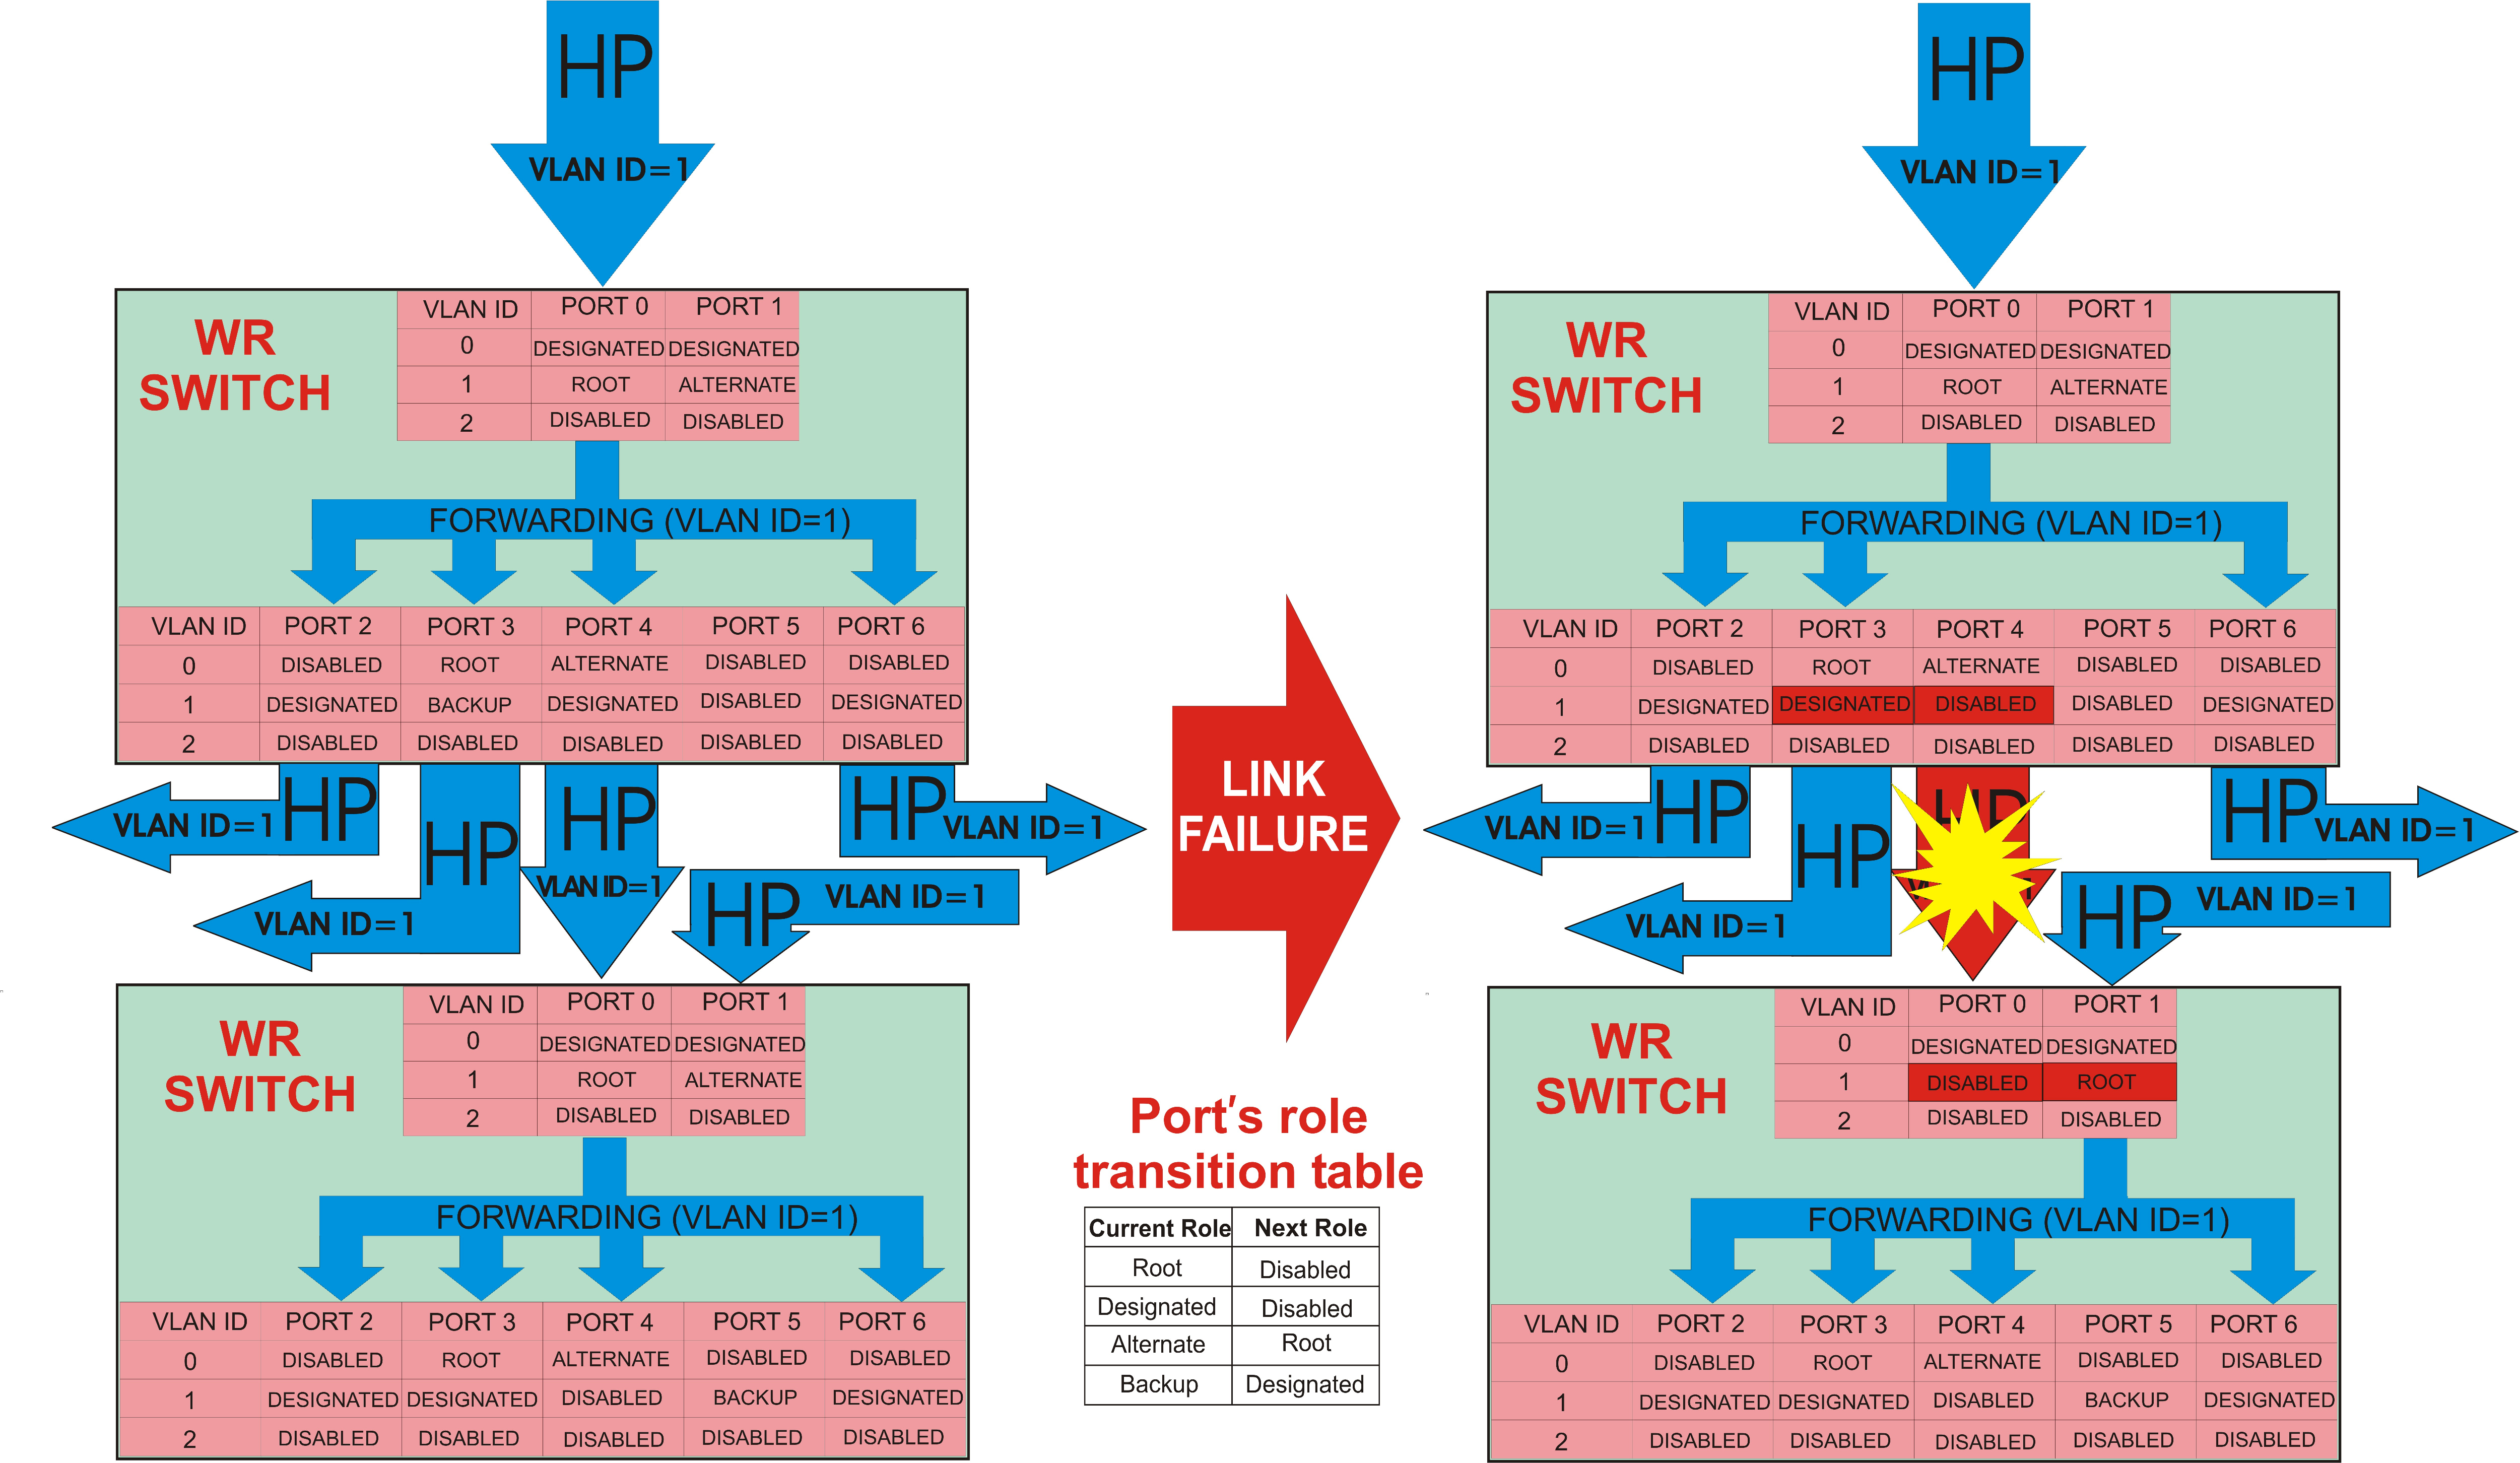
\includegraphics[scale=0.20]{robustness/wrRSTP.ps}
	\captionof{figure}{WR RSTP for HP Traffic}
	\label{fig:wrRSTP}
\end{center}

\chapter{Appendix: Rapid Spanning Tree and White Rabbit}
\label{appD}

\section{Rapid Spanning Tree}

The end goal of STP is to ensure that only one port of a switch is responsible 
for forwarding traffic from the direction of the Root Switch onto any given
link. In networks running STP, every bridge has a priority value associated with
it, according with this value, the switch with the lowest priority will become
the Root of the network.  This process is done by the exchange of BPDUs packets
(Bridge Protocol Data Units) between switches. The rest of the switches shall be
Designated Switched, which forwards packets from the LAN toward the root bridge,
and vice versa.

\begin{center}
        \includegraphics[scale=0.20 ]{robustness/network_beginning.pdf}
        \captionof{figure}{Redundant Network with Loops}
        \label{fig:redunt_net}
\end{center}


Once that the Root Switch has been defined, the switches shall determine
the least cost paths to the Root Switch. The cost is based on the number of
links from the switch till the root, and the cost of every link is based on the
Data Rate of the link. Data Rate ref(table of "Data rate and STP path cost"). In
case that two path have the same cost, there is a mechanism for breaking the
tie.

\begin{itemize}
        \item Root Port: provides connectivity to the root bridge
        \item Designated Port: forwards traffic from the root port onto the
next link.
        \item Alternate Port: an alternate path to the root bridge.
        \item Backup Port: a backup/redundant link to a segment where
another bridge port already connects.
\end{itemize}


RSTP implements distributed variation of Bellman-Ford iterative
algorithm, which could be described as "gradient" process, meaning it iteratively looks for the
optimal solution, selecting an "optimal" candidate every time. Every switch
(with except to the root) send and  accepts BPDU packets
with its information. The switch retains only the best current Root Switch
information electing one root port upstream toward the root switch. The switch
then block alternate paths to the root switch, leaving only the single optimal
upstream path and continue relaying optimal information downstream. If a switch
learns of a better root switch, on any of its ports, the previous "best"
information is erased and the new one immediately accepted and relayed. This
proccess will be propagated to all the switches, and it leads to the convergence
of the network where only one switch will be identified as root, and the rest of
the switches as designated with one port as Root Port and the rest Designated,
Alternate or Backup Port.


\begin{center}
        \includegraphics[scale=0.20 ]{robustness/network_spanning.pdf}
        \captionof{figure}{Free-Loops Network}
        \label{fig:free_loops}
\end{center}

The process of initial convergence it's not crucial for time
critical application, since it will be issued once the network is switched on.
Conversely, how ST deal with topologies changes and its
convergence, is extremely important for time critical application, like WR where
the packets tagged with the highest priority convey Control Information that
should not be lost due to a change of topology.

Normally, when a switch detects a topology change, it issues BDPU packets with
the Topology Change bit set. Every bridge that receives a BPDU with TC flag set,
should  receive it on either root port (coming from upstream) or designated port
(coming from downstream). The receiving bridge performs the following:
\begin{itemize}

        \item Flushes all MAC addresses associated with all ports with except to
the port where the TC BPDU was received
        \item Repeats the flooding procedure by starting Topology Change timer
and setting the TC bit for all BPDUs sent upstream or downstream. The receiving
port is excluded from flooding, in order to ensure flooding procedure
termination.
\end{itemize}
and the convergence process stars for this topology change. 



The end goal of STP is to ensure that only one port of a switch is responsible 
for forwarding traffic from the direction of the Root Switch onto any given
link. In networks running STP, every bridge has a priority value associated with
it, according with this value, the switch with the lowest priority will become
the Root of the network.  This process is done by the exchange of BPDUs packets
(Bridge Protocol Data Units) between switches. The rest of the switches shall be
Designated Switched, which forwards packets from the LAN toward the root bridge,
and vice versa.

\begin{center}
        \includegraphics[scale=0.20 ]{robustness/network_beginning.pdf}
        \captionof{figure}{Redundant Network with Loops}
        \label{fig:redunt_net}
\end{center}


Once that the Root Switch has been defined, the switches shall determine
the least cost paths to the Root Switch. The cost is based on the number of
links from the switch till the root, and the cost of every link is based on the
Data Rate of the link. Data Rate ref(table of "Data rate and STP path cost"). In
case that two path have the same cost, there is a mechanism for breaking the
tie.

\begin{itemize}
        \item Root Port: provides connectivity to the root bridge
        \item Designated Port: forwards traffic from the root port onto the
next link.
        \item Alternate Port: an alternate path to the root bridge.
        \item Backup Port: a backup/redundant link to a segment where
another bridge port already connects.
\end{itemize}


RSTP implements distributed variation of Bellman-Ford iterative
algorithm, which could be described as "gradient" process, meaning it iteratively looks for the
optimal solution, selecting an "optimal" candidate every time. Every switch
(with except to the root) send and  accepts BPDU packets
with its information. The switch retains only the best current Root Switch
information electing one root port upstream toward the root switch. The switch
then block alternate paths to the root switch, leaving only the single optimal
upstream path and continue relaying optimal information downstream. If a switch
learns of a better root switch, on any of its ports, the previous "best"
information is erased and the new one immediately accepted and relayed. This
process will be propagated to all the switches, and it leads to the convergence
of the network where only one switch will be identified as root, and the rest of
the switches as designated with one port as Root Port and the rest designated,
Alternate or Backup Port.


\begin{center}
        \includegraphics[scale=0.20 ]{robustness/network_spanning.pdf}
        \captionof{figure}{Free-Loops Network}
        \label{fig:free_loops}
\end{center}

The process of initial convergence it's not crucial for time
critical application, since it will be issued once the network is switched on.
Conversely, how ST deal with topologies changes and its
convergence, is extremely important for time critical application, like WR where
the packets tagged with the highest priority convey Control Information that
should not be lost due to a change of topology.

Normally, when a switch detects a topology change, it issues BDPU packets with
the Topology Change bit set. Every bridge that receives a BPDU with TC flag set,
should  receive it on either root port (coming from upstream) or designated port
(coming from downstream). The receiving bridge performs the following:
\begin{itemize}

        \item Flushes all MAC addresses associated with all ports with except to
the port where the TC BPDU was received
        \item Repeats the flooding procedure by starting Topology Change timer
and setting the TC bit for all BPDUs sent upstream or downstream. The receiving
port is excluded from flooding, in order to ensure flooding procedure
termination.
\end{itemize}
and the convergence process stars for this topology change. 

\subsection{Convergence in RSTP}

When a RSTP bridge detects a topology change by missing same BPDU seconds
(\textsl{Max Age Message}). Depending on the port state, the protocol will
handle the failure differently: 

\begin{itemize}

	\item If the port was blocking, nothing happens with except to expiring 
information associated with the failed port.
	\item If the port was designated, does nothing. However, downstream
switch may detect the loss of a root port and start converging. 
	\item If the port was a root: 

	\begin{itemize}
		\item It starts the  timer with a value equal to twice the 
hello-time (ref) for all its designated ports and its root port, if necessary.
		\item It flushes the MAC addresses associated with all these
ports.
	\end{itemize}

\end{itemize}


When a switch receives a BPDU with the TC bit set from a neighbor:

\begin{itemize}
 
	\item It clears the MAC addresses learned on all its ports, except the 
one that receives the topology change. 
	\item It starts the timer and sends BPDUs with Topoloy Change set on all
 its designated ports and root port.
\end{itemize}

This way, the Topology Change Notification floods very quickly across the whole 
network. The Topology Change propagation is now a one step process. In fact, the
initiator of the topology change floods this information throughout the network.

In just a few seconds, or a small multiple of hello-times, most of the entries 
in the routing tables of the entire network flush. This approach results in
potentially more temporary flooding, but on the other hand it clears potential
stale information that prevents rapid connectivity restitution. 



\textbf{Convergence in Dual Link Topology}

The Dual Link Topology a particular case of fast recovery. Both switches detects
 failure of a link  simultaneously and immediately age out the learned MAC
address entries for these ports. Bridge B has been receiving periodic
transmissions of BPDUs on the other link. This information allows it to evaluate
the second link as its best path to the to the root bridge. Bridge B immediately
sets its root port. 

RSTP procedure requires a topology change when adding a path to the topology. 
Bridge B "sees" the new root port as an added path and floods topology changes
out its ports. Though not strictly necessary in this case, they cause no ill
effects.

\begin{center}
        \includegraphics[scale=0.70 ]{robustness/dual_link.pdf}
        \captionof{figure}{Convergence Dual Link Topology}
        \label{fig:idual_link}
\end{center}

\textbf{Convergence in case of Root Port Loss}

The switch C  detects loss of the root port, by missing BPDUs for same time 
(e.g. 3xHello time). Next, the following is the sequence of events that occurs:

The switch C declares loss of the root bridge. Since the switch has no other 
paths to the root, it declares
itself as the new root bridge for the topology and attempts to synchronize  this
information with the rest of 
the topology. The synchronization wave will propagate through Switch B and 
eventually reaches D, which has better root port information. The sync wave
bounces back and goes till C to adapt to the new information and will declare
the designated port as root port.

\begin{center}
        \includegraphics[scale=0.70 ]{robustness/indirect_change_explamation.pdf}
        \captionof{figure}{Convergence Indirect Change of Topology}
        \label{fig:indirect_change}
\end{center}

\section{White Rabbit RSTP Use Cases}

\begin{center}
	\includegraphics[scale=0.40]{robustness/WRRSTPforHP.pdf}
	\captionof{figure}{Some topology of the network and the bit we are
considering.}
	\label{fig:WRRSTPforHP}
\end{center}

\begin{center}
	\includegraphics[scale=0.40]{robustness/WRRSTPforHP2.pdf}
	\captionof{figure}{The considered fragment of the network.}
	\label{fig:WRRSTPforHP2}
\end{center}

\begin{center}
	\includegraphics[scale=0.40]{robustness/WRRSTPcase1.pdf}
	\captionof{figure}{Link failure Use Case.}
	\label{fig:WRRSTPcase1}
\end{center}

\begin{center}
	\includegraphics[scale=0.40]{robustness/WRRSTPcase2.pdf}
	\captionof{figure}{Switch failure Use Case.}
	\label{fig:WRRSTPcase2}
\end{center}
\begin{center}
	\includegraphics[scale=0.40]{robustness/WRRSTPcase3.pdf}
	\captionof{figure}{Link failure Use Case.}
	\label{fig:WRRSTPcase3}
\end{center}

\begin{center}
	\includegraphics[scale=0.40]{robustness/WRRSTPcase4.pdf}
	\captionof{figure}{Failure of the switch connected to Data Master Node
(assuming flawless switching to backup Data Master.}
	\label{fig:WRRSTPcase4}
\end{center}

\begin{center}
	\includegraphics[scale=0.40]{robustness/WRRSTPcase5.pdf}
	\captionof{figure}{Link Failure between switches connected to
Master Node and backup Master Node}
	\label{fig:WRRSTPcase5}
\end{center}

\section{Solutions to overcome RSTP limitations}
The proposed solution has its limitation, to overcome this shortcomings, three
solutions are considered:
\begin{itemize}
  \item Map/Table of possible changes of topology in each
switch + WR BPDU, in HW (Non-Standard). 
  \item WR BPDU + using RSTP data + some additional logic, in HW (Non-standard,
).
  \item WR BPDU + using RSTP data + some additional logic, in HW
(Almost-standard).
\end{itemize}
They are not to be described in details in the first release of the document,
these are exceptional/rare cases.

\chapter{Appendix: Potential Modifications to RTU required by RSTP}
\label{appE}

Potential changes to RTU needed by RSTP: \\
1. RTU@HW:
\begin{itemize}
  \item Blocking of incoming packages per-VLAN (currently only per-port).
  \item Blocking of outcoming packages per-port (currently only per-VLAN).
\end{itemize}
2. RTU@SW:
\begin{itemize}
  \item aging of information on a given port - this means queuing Filtering
Database for the entries belonging to given port, and removing (aging out) this
entries).
  \item changes enabling control of new HW parameters.
\end{itemize}
\chapter{Appendix: Forward Error Correction}
\label{appFEC}
\section{Hamming Code}

Hamming Code/Decode algorithm 

In a Hamming code parity-check bits are added to the original message bits. Any bit, whether the bits of the origninal messege or the parity-check bits, 
would have a unique combination of check-bits associated with it. The original-bits and the parity-check bits are spoted at particular locations in
the frame, the pattern is followed in any Hamming Code and no matter how many check-bits are included. The parity bit $c_i$ is used to convey the parity 
bit for all bits in the code whose position have a binary representation with a $1$ in position $i$. The Table ~ref{tab:HAMING} presents 

\begin{table}[!ht]
        \begin{center}
                \begin{tabular}{|c c|c|c|c|c|c|c|c|c|c|c|c|c|c|c|c|c|}
\hline
Bit Position & & 1 & 2 & 3 & 4 & 5 & 6 & 7 & 8 & 9 & 10 & 11 & 12 & 13 & 14 & 15 & 16  \\ \hline
%Encoded data Bit 

\multicolumn{2}{|c|}{Encoded data Bit } & \colorbox{green}{p1}	& \colorbox{green}{p2} &	d1 &	\colorbox{green}{p4}	& d2 &	d3 &	d4 &	\colorbox{green}{p8} &	d5 & d6 &	d7 &	d8 &	d9 &	d10 &	d11 &	\colorbox{green}{p16}  \\ \hline

\multirow{5}{*}{Paritiy Bit} 
		 & \multicolumn{1}{|c|}{\colorbox{green}{p1}} & X &  & X &  & X &  & X &  & X &  &X &  &X&  &X &  \\ \cline{2-18}%
		 & \multicolumn{1}{|c|}{\colorbox{green}{p2}} & & X &X & & & X& X& & &X &X & & &X &X &  \\  \cline{2-18}%
		 & \multicolumn{1}{|c|}{\colorbox{green}{p4}} & & & &X &X &X &X & & & & &X &X &X &X &   \\  \cline{2-18}%
		 & \multicolumn{1}{|c|}{\colorbox{green}{p8}} & & & & & & & &X &X &X &X &X &X &X &X &   \\  \cline{2-18}%
		 & \multicolumn{1}{|c|}{\colorbox{green}{p16}} & & & & & & & & & & & & & &  & & X  \\ \hline

        	\end{tabular}
          \caption{Postion of the parity-check bits and Information bits in a Hamming Code}
	  \label{tab:HAMING}
	\end{center} 
\end{table}

The parity bits are calculate as follows:

\begin{table}[!ht]
        \begin{center}
                \begin{tabular}{c c c c c c c c c c c c c c c c c}
	         p1= & d1 &$\oplus$& d2 &$\oplus$&    &$\oplus$& d4 &$\oplus$& d5 &          &    &$\oplus$& d7 &          &     \\
		 p2= & d1 &        &    &$\oplus$& d3 &$\oplus$& d4 &$\oplus$&    & $\oplus$ & d6 &$\oplus$& d7 &          &      \\
	         p4= &    &        &    &        &    &        &    &$\oplus$& d5 & $\oplus$ & d6 &$\oplus$& d7 & $\oplus$ & d8   \\
... = & .... &&&&&&&&&&& \\
	
		 		\end{tabular}   
	\end{center}
\end{table}

The decoding process will calculate the parity-check bits again 

\begin{table}[!ht]
        \begin{center}
                \begin{tabular}{c c c c c c c c c c c c c c c c c}
	         p1'= & d1 &$\oplus$& d2 &$\oplus$&    &$\oplus$& d4 &$\oplus$& d5 &          &    &$\oplus$& d7 &          &     \\
		 p2'= & d1 &        &    &$\oplus$& d3 &$\oplus$& d4 &$\oplus$&    & $\oplus$ & d6 &$\oplus$& d7 &          &      \\
	         p4'= &    &        &    &        &    &        &    &$\oplus$& d5 & $\oplus$ & d6 &$\oplus$& d7 & $\oplus$ & d8   \\
... = & .... &&&&&&&&&&& \\
	
		 		\end{tabular}   
	\end{center}
\end{table}

The exclusive-or operation between the received parity-check  bits: p1,p2 etc.. and the calculate parity-check  bits: p1',p2' etc... 

\begin{table}[!ht]
        \begin{center}
                \begin{tabular}{cccc}
         e1 = & p1 &$\oplus$& p1' \\
				 e2 = & p2 &$\oplus$& p2' \\
			   e3 = & p4 &$\oplus$& p4' \\
				... = & ....  &$\oplus$& .... \\
		 		\end{tabular}   
	\end{center}
\end{table}

will indicate no error in the frame if all $e_i$ are 0, otherwise the value indicate the position of error in the frame, and it shall be correct by flipping the received value.


%%%%%%%%%%%%%%%%%%%%%%%%%%%%%%%%%%%%%%%%%%%%%%%%%%%%%%%%%%%%%%%%%%%%%%
\section{Reed Solomon}

Reed Solomon encoding and decoding is based on the domain of Galois  field $GF(2^m)$.  The value, m, is the code word size of the encoding. 
The \ControlMessage is subdivided into code blocks of length $m$ bits and check values must be computed for each code block. 
The frames transmitted consists of \ControlMessage frames and check frames used in reconstructing lost frames. 

The algorithm requires an encoding/decoding matrix of $n+k$ rows and n columns
with following properties:


\begin{itemize}
    \item Identity Matrix Property: the first $n$ rows constitute a $n \times n$ identity matrix, $I$. 
    \item Independent Linearity: any n of the $n+k$ rows are linearly independent. This property ensures that any collection of exactly $n$ rows constitutes an invertible $n \times $ matrix.

The required matrix for encoding is derived from Vandermonde matrix. For arbitrary n and m, this matrix has the following form. The fact
that the largest value in $GF(2^m)$ is $2^m-1$ necessarily constrains the number of rows and columns in the matrix $(n + k)$ to be less than or equal to $2^m$
\end{itemize}

\vspace{0.5cm}
\begin{center}
$V= 
\begin{bmatrix} 

0^0 & 0^1 & 0^2 & .... & 0^{(n-1)} \\ 
1^0 & 1^1 & 1^2 & .... & 1^{(n-1)} \\
2^0 & 2^1 & 2^2 & .... & 2^{(n-1)} \\ 
... & ... & ... & .....& ...	   \\
(2^m-1)^0 & (2^m-1)^1 & (2^m-1)^2 & .... & (2^m-1)^{(n-1)} \\

\end{bmatrix}$
\end{center}
\vspace{0.5cm}

This matrix $V$ doesn't possess property of idependant linearity, but clearly
does not possess the identity matrix. Nevertheless, by a series of linear transformations in which a multiple of one
column is added to another, we can obtain a matrix with the identity matrix
property  while preserving the independence of the vectors. We will call this transformed matrix $D$.

\vspace{0.5cm}
\begin{center}
$D= 
\begin{bmatrix} 

1 & 0 & 0 & .... & 0 \\ 
0 & 1 & 0 & .... & 0  \\
0 & 0 & 1 & .... & 0 \\ 
... & ... & ...  & .....& ....\\
0 & 0 & 0 & .... & 1\\ 
a & b & c & .... & d \\
a_1 & b_1 & c_1 & .... & d_1 \\
a_2 & b_2 & c_2 & .... & d_2 \\
a_3 & b_3 & c_3 & .... & d_3 \\
... & ... & ...  & .....& ....\\
a_{n-1} & b_{n-1} & c_{n-1} & .... & d_{n-1} \\

\end{bmatrix}$
\end{center}
\vspace{0.5cm}


The bottom $k$ rows of the transformed Vandermonde matrix, $D$, constitute the encoding matrix $E$ that is used to create the $k$ check frames. The matrix $E$ has dimension $k \times n$ where $k$ is the number of check frames and $n$ is the number of \ControlMessage frames. When the $n \times 1$ vector of code block is multiplied by $E$ the check values is produced. The encoding algorithm each code word is $b$ bits. If an actual \ControlMessage consisted of 4000 $b$ bits, the process described above would have to be repeated 4000 times, once for each code block in the \ControlMessage.
\vspace{0.5cm}

\begin{center}
$E= 
\begin{bmatrix} 
a   & b   & c   & ... & d		\\
a_1 & b_1 & c_1 & ... & d_1 \\
a_2 & b_2 & c_2 & ... & d_2 \\
a_3 & b_3 & c_3 & ... & d_3 \\
... & ... & ... & ... & ...\\
a_{n-1} & b_{n-1} & c_{n-1} & ... & d_{n-1}
\end{bmatrix}$
\end{center}

\vspace{0.5cm}

\begin{center}
$
\begin{bmatrix} 
a   & b   & c   & ... & d   \\
a_1 & b_1 & c_1 & ... & d_1 \\
a_2 & b_2 & c_2 & ... & d_2 \\
a_3 & b_3 & c_3 & ... & d_3 \\
... & ... & ... & ... & ... \\
a_{n-1} & b_{n-1} & c_{n-1} & ... & d_{n-1} 
\end{bmatrix}
$
$\times$
$
\begin{bmatrix} 
bit \\ bit_1 \\ bit_2 \\ bit_3 \\...\\bit_{n-1} 
\end{bmatrix} 
$
$=$
$
\begin{bmatrix} 
ebit \\ ebit_1 \\ ebit_2 \\ ebit_3 \\ ... \\ ebit_{n-1} 
\end{bmatrix}
$
\end{center}

\vspace{0.5cm}

The decoding algorithm supposes a collection of n frames including both \ControlMessage  and check frames have been received. 
We extract the n rows of the matrix corresponding the $n$ received packets. We call this $n \times n$ matrix $D'$. We invert $D'$ to obtain $D'^{-1}$.
Then the product of $D'^{-1}$ and the received mixture of data words and check words recovers the data words $d0, ...d_{n-1}$.

\begin{center}
$D'=
\begin{bmatrix} 
a   & b   & c   & ... & d   \\
a_1 & b_1 & c_1 & ... & d_1 \\
a_3 & b_3 & c_3 & ... & d_3 \\
... & ... & ... & ... & ... \\
a_{n-1} & b_{n-1} & c_{n-1} & ... & d_{n-1} 
\end{bmatrix}
$
\end{center}
\vspace{0.5cm}

\begin{center}
$
\begin{bmatrix} 
a   & b   & c   & ... & d   \\
a_1 & b_1 & c_1 & ... & d_1 \\
a_3 & b_3 & c_3 & ... & d_3 \\
... & ... & ... & ... & ... \\
a_{n-1} & b_{n-1} & c_{n-1} & ... & d_{n-1} 
\end{bmatrix}
$
$\times$
$
\begin{bmatrix} 
ebit \\ ebit_1  \\ ebit_3 \\ ... \\ ebit_{n-1} 
\end{bmatrix}
$
$=$
$
\begin{bmatrix} 
a \\ b \\ c \\ ... \\ z 
\end{bmatrix}
$
\end{center}
\vspace{0.5cm}
Because the receiver also knows the algorithm by which the check frames were constructed, inverting $D'$ yields $D'^{-1}$. Multiplying the received check values by $D'{-1}$ recovers the original values.

\begin{center}
$D'^{-1}$ 
$\times$
$
\begin{bmatrix} 
a \\ b \\ c \\ ... \\ z 
\end{bmatrix}
$
$=$
$
\begin{bmatrix} 
bit \\ bit_1 \\ bit_2 \\ bit_3 \\...\\bit_{n-1} 
\end{bmatrix} 
$
\end{center}

Error recovery inverts the $n \times n$ matrix composed of rows from the $D$ matrix corresponding to the $n$ frames encoded that were
actually received. In the worse case this inversion is $O(n^3)$ . The cost of
the inversion is proportional to the number of check rows that must be replaced
in the identity rows in the decode matrix. When the inversion has been completed,
it is necessary to multiply the received vector of $n$ block code by the $n \times n$ inverse matrix for each block code in the frame. 


%%%%%%%%%%%%%%%%%%%%%%%%%%%%%%%%%%%%%%%%%%%%%%%%%%%%%%%%%%%%%%%%%%%%%%%
\section{White Rabbit FEC Graphs}
\label{app:wr_fec_graphs}


\subsection{WR FEC Graps in  CERN Network}

\begin{center}
        \includegraphics[scale=0.60]{../../../../figures/robustness/P_error_control_msg_CERN.ps}
        \captionof{figure}{Probability of Losing a Control Message}
         \label{fig:wrRSTPtopologies}
\end{center}

The Figure ~\ref{fig:wrRSTPtopologies} compares the FEC scheme proposed with a simple repetition code.


\begin{center}
        \includegraphics[scale=0.60]{../../../../figures/robustness/overhead_cern.ps}
        \captionof{figure}{Overhead introduced by the WR FEC Scheme}
         \label{fig:wrRSTPtopologies}
\end{center}



\subsection{WR FEC Graps in  GSI Network}


\begin{center}
        \includegraphics[scale=0.60]{../../../../figures/robustness/P_error_control_msg_GSI.ps}
        \captionof{figure}{Probability of Losing a Control Message}
         \label{fig:wrRSTPtopologies}
\end{center}


The Figure ~\ref{fig:wrRSTPtopologies} compares the FEC scheme proposed with a simple repetition code.

\begin{center}
        \includegraphics[scale=0.60]{../../../../figures/robustness/overhead_gsi.ps}
        \captionof{figure}{Overhead introduced by the WR FEC Scheme}
         \label{fig:wrRSTPtopologies}
\end{center}

\label{app:wr_fec_Graphs}










\chapter{Appendix: Timing and Prioritizing of the Ideas Presented} 
\label{appF}

The number of ideas presented in this document is overwhelming. Not all the
ideas are necessary for White Rabbit to work as Control Network
which is carefully controlled, managed and configured. Some of the ideas are
thought for the more general usage. The below table attempts to prioritize the
ideas, group it into areas and present planning.


\begin{table}[ht]
\caption{Timing and Prioritizing of the Ideas Presented.} 
\centering
\begin{tabular}{| p{3.5cm} | p{1cm} | p{3.5cm} | p{1.5cm} | p{3.5cm} |} \hline
\textbf{Name}&\textbf{Prio}& \textbf{Approx. finished}&\textbf{Ref
Chapter} & \textbf{Area}  \\ \hline
FEC       & 1  & Workshop April 2011 & \ref{chapter:FEC} & Control Data\\ \hline
HP Bypass & 2  & Workshop after April Workshop & \ref{chapter:FEC} & Control
Data\\ \hline
WR RSTP (HP only)   & 2  & Workshop after April Workshop& \ref{chapter:WRRSTP} &
Control,
Standard Data and a bit timing     
\\ \hline
Monitoring (limited) & 2  & Workshop after April Workshop &
\ref{chapter:monitoring} &
Diagnostics, Monitoring   
\\ \hline \hline
Congestion/Flow Control & 3  & 2012 & \ref{chapter:monitoring} &
Standard and Control Data   
\\ \hline
Management & 3  & 2012 & \ref{chapter:monitoring} &
Standard and Control Data   s
\\ \hline
Full Monitoring & 3  & 2012 & \ref{chapter:monitoring} &
Diagnostics
\\ \hline \hline
Transparent Clocks PTP & 4  & ? & - & Timing Data
\\ \hline
Ring topologies      & 5  & ? & - & Timing and Control Data Earthquake 
\\ \hline
%Congestion/flow control, standard and for all the priorities      & 5  & ? & -
%&
%Control Data
%\\ \hline
Link Aggregation & 5  & ? & - & Timing, Control and Standard Data
\\ \hline
WR RSTP (SP traffic and other crazy ideas regarding SP and HP)   & 6  &  ? &
\ref{chapter:WRRSTP} &
Control and Standard Data
\\ \hline


\end{tabular}
\label{tab:RobustnessPrioAndPlan}
\end{table}

\chapter{Appendix:Flow Monitor} 
\label{appSFlow}

\section{sFlow}

sFlow is a multi-vendor sampling technology embedded within switches and
routers. It provides the ability to continuously monitor application level
traffic flows at wire speed on all interfaces
simultaneously~\ref{tab:sflow_info}.


sFlow consists of:

\begin{itemize}
	\item sFlow Agent 
	\item sFlow Collector
\end{itemize}

The sFlow Agent is a software process that runs in the White Rabbit Switches.
 It combines interface Counters and Flow Samples into sFlow datagrams that are
sent across the network to an sFlow Collector. The Counters and Flow Samples
will be implemented in hardware in order to increase the
processing of the data sampling. Flow samples are defined based on a sampling
rate, an average of 1 out of N packets is randomly sampled. This type of
sampling provides  quantifiable accuracy. A polling interval defines how often
the network device sends interface counters. 

The sFlow Agent packages the data into sFlow Datagrams that are sent on the
network. The sFlow Collector receives the data from the Flow generators, stores
the information and provides reports and analysis. 

\subsubsection{Configuration}

Every switch capable of sFlow must configure and enable:

\begin{itemize}
	\item local agent
	\item sFlow Colector address 
	\item ports to monitor
\end{itemize}

In order to acquire a reliable network information in a WR network:

\begin{itemize}
	\item the statistics shall be collected every ?? (sec,msec..)
	\item a sample is taken per port every ?? (sec,msec...)
	\item ?? samples per port shall be sent to the CPU

\end{itemize}


\section{Requirements of a Flow Monitor}

General requirements:
\begin{itemize}
	\item Network-wide view of usage and active switches. 
	\item Measuring network traffic, collecting, storing, and analysing
traffic data.
	\item Monitor links without impacting the performance of the switches
without adding significant network load.
	\item Industrial Standard
\end{itemize}

\noindent The Flow Monitor shall: 

\begin{itemize}
	\item Measure the volume and rate of the traffic by QoS level.
	\item Measure the availability of the network and devices.
	\item Measure the response time that a device takes to react to a given
input.
	\item Measure the throughput of the over the links.
	\item Measure the latency and jitter of the network.	
	\item Identify grouping of traffic by logics groups (Master, Node,
Switch)
	\item Identify grouping of traffic by protocols.
	\item Define filters and exceptions associated with alarms and
notification.
\end{itemize} 


\noindent The measurements shall be carried out either between network devices,

\noindent Per-Link Measurements, and monitor:

		\begin{itemize}	
			\item number of packet
			\item bytes
			\item packet discarded on an interface
			\item flow or burst of packets
			\item packets per flow
		\end{itemize}

\noindent or End-to-End Measurements:
		\begin{itemize}	
			\item path delay  
			\item ....
			\item ....
		\end{itemize} 

\noindent The combination of both measurements provides a global picture of the
network.


\vspace{10 mm}

\noindent The monitoring shall performance:

\begin{itemize}
	\item Active Measurement, injection of network traffic and study the
reaction to the traffic
	\item Passive Measurement,  Monitor of the traffic for measurement.
\end{itemize}

\vspace{10 mm}

\noindent Performance:

\begin{itemize}

	\item Reaction Time ... 
	\item Sampling...
	
\end{itemize}


\section{State of the Art of Flow Controller}

Currently there are three main choices for traffic monitoring:

\begin{itemize}

	\item RMON, IETD standard.
	\item NetFlow, Cisco Systems.
	\item sFlow, Industry standard
\end{itemize}

In a nutshell, all them offers the similar features and provides the same
information, thus the selection criteria is based on the usage of resources by
the Agent in the switches and the collector of information.

\begin{table}[ht]
\begin{center}
    \begin{tabular}{ | c | c | c | c | c | c | c |}
\hline
Flow Controllers & CPU & Memory & Bandwidth & RT Statistics & Implementation \\
\hline
RMON & high &  very high 8-32 MB & bursty & supported & sw \\ \hline
NetFlow & high & high 4-8 MB & high bursty & not & sw  \\ \hline
sFlow & very low & very low akB & low smooth & supported & sw/hw \\ \hline
    \end{tabular}
\end{center}
\caption{Comparison Flow Control}
\end{table}

As the Table~\ref{tab:flow_controlers} shows that sFlow requires less resources
either in the Agent, which is placed in the switch, or the Collector. As well
the usage of bandwidth is more conservative since the gathered information every
short periods of time, conversely to the others controllers. It seems that
sFlows becomes a good choice for White Rabbit. Besides sFlows allows the
implementation of part of Agent in hardware, providing wire-speed to the
sampling of frames. In addition the license scheme of sFlow's  allows White
Rabbit project modify and publish our own version.


\chapter{Appendix: WR-specific MIB definitions} 
\label{appG}

\section{WR PTP}
\vspace{5 mm}
\textbf{All applicable data sets} \\
\vspace{5 mm}
SYNTAX INTEGER {
\begin{table}[!ht]
%\begin{center}
\scriptsize 
\begin{tabular}{ l l }
\textbf{ps1(23),}   & \textbf{-- The time is accurate to 1ps} \\
\textbf{ps2p5(24),} & \textbf{-- The time is accurate to 2.5ps} \\
\textbf{ps10(25),}  & \textbf{-- The time is accurate to 10ps} \\
\textbf{ps25(26),}  & \textbf{-- The time is accurate to 25ps} \\
\textbf{ps100(27),} & \textbf{-- The time is accurate to 100ps} \\
\textbf{ps250(28),} & \textbf{-- The time is accurate to 250ps} \\
\textbf{ns1(29),}   & \textbf{-- The time is accurate to 1ns} \\
\textbf{ns2p5(30),} & \textbf{-- The time is accurate to 2.5ns} \\
\textbf{ns10(31),}  & \textbf{-- The time is accurate to 10ns} \\
ns25(32),   & -- The time is accurate to 25ns \\
ns100(33),  & -- The time is accurate to 100ns \\
ns250(34),  & -- The time is accurate to 250ns \\
us1(35),    & -- The time is accurate to 1us \\
us2p5(36),  & -- The time is accurate to 2.5us \\
us10(37),   & -- The time is accurate to 10us \\
us25(38),   & -- The time is accurate to 25us \\
us100(39),  & -- The time is accurate to 100us \\
us250(40),  & -- The time is accurate to 250us \\
ms1(41),    & -- The time is accurate to 1ms \\
ms2p5(42),  & -- The time is accurate to 2.5ms \\
ms10(43),   & -- The time is accurate to 10ms \\
ms25(44),   & -- The time is accurate to 25ms \\
ms100(45),  & -- The time is accurate to 100ms \\
ms250(46),  & -- The time is accurate to 250ms \\
s1(47),     & -- The time is accurate to 1s \\
s10(48),    & -- The time is accurate to 10s \\
s10plus(49) & -- The time is accurate to >10s \\
\end{tabular}
%\end{center}
\end{table}
}
\newline
\vspace{5 mm}
\textbf{Parent Data Set}  \\
\vspace{5 mm}
wrptpGrandmasterWrPortMode OBJECT-TYPE \\
SYNTAX INTEGER \{ \\
\tab NON\_WR (0), \\
\tab WR\_SLAVE (1), \\
\tab WR\_MASTER(2), \\
\} \\
MAX-ACCESS read-only \\
STATUS current \\
DESCRIPTION \\
"Determines predefined function of the PTP grandmaster."  \\
REFERENCE \\
"WR Spec: Clause 6.2, Table 1" \\
::= { ptpParentDataSet 10 } \\
\\
wrptpGrandmasterDeltaTx OBJECT-TYPE \\
SYNTAX INTEGER \\
MAX-ACCESS read-only \\
STATUS current \\
DESCRIPTION \\
Grandmaster's $\Delta_{tx}$ measured in picoseconds and multiplied by $2^{16}$ .
REFERENCE  \\
"WR Spec: Clause 6.2, Table 1" \\
::= { ptpParentDataSet 11 } \\
\\
wrptpGrandmasterDeltaRx OBJECT-TYPE \\
SYNTAX INTEGER \\
MAX-ACCESS read-only \\
STATUS current \\
DESCRIPTION \\
"Grandmaster's $\Delta_{rx}$ measured in picoseconds and multiplied by
 $2^{16}$."  \\
REFERENCE  \\
"WR Spec: Clause 6.2, Table 1" \\
::= { ptpParentDataSet 12 } \\
\\
wrptpGrandmasterDeltaRx OBJECT-TYPE
SYNTAX TruthValue
MAX-ACCESS read-only
STATUS current
DESCRIPTION
"If TRUE, the grandmaster is working in WR mode."
REFERENCE
"WR Spec: Clause 6.2, Table 1"
::= { ptpParentDataSet 13 }
\vspace{5 mm}
\textbf{Port Data Set} \\
\vspace{5 mm}

wrptpPortState OBJECT-TYPE \\
SYNTAX INTEGER \{ \\
\tab idle(1), \\
\tab present(2), \\
\tab m\_lock(3), \\
\tab s\_lock(4), \\
\tab locked(5), \\
\tab req\_calibration(6), \\
\tab calibrated(7), \\
\tab resp\_calib\_req(8), \\
\tab wr\_link\_on(9) \} \\
MAX-ACCESS read-only \\
STATUS current \\
DESCRIPTION \\
"White Rabbit State Machine." \\
REFERENCE \\
"WR Spec: Clause 6.5.2.1" \\
DEFVAL { idle } \\
::= { ptpPortDataSet 11 } \\
\\
wrptpPortState OBJECT-TYPE  \\
SYNTAX INTEGER \{ \\
\tab NON\_WR (0), \\
\tab WR\_SLAVE (1), \\ 
\tab WR\_MASTER(2), \\
\} \\
MAX-ACCESS read-only \\ 
STATUS current \\
DESCRIPTION \\
"Determines predefined function of WR port (static)." \\
REFERENCE \\
"WR Spec: Clause 6.2, Table 1" \\
::= { ptpPortDataSet 12 } \\
\\
wrptpCalibrated OBJECT-TYPE \\
SYNTAX TruthValue \\
MAX-ACCESS read-only \\
STATUS current \\
DESCRIPTION \\
"Indicates whether fixed delays of the given port are known." \\
REFERENCE \\
"WR Spec: Clause 6.2, Table 1" \\
::= { ptpPortDataSet 13 } \\
\\
wrptpDeltaTx OBJECT-TYPE  \\
SYNTAX INTEGER \\
MAX-ACCESS read-only \\
STATUS current \\
DESCRIPTION \\
"Port's $\Delta_{tx}$ measured in picoseconds and multiplied by $2^{16}$." \\
REFERENCE \\
"WR Spec: Clause 6.2, Table 1" \\
::= { ptpPortDataSet 14 } \\
\\
wrptpDeltaRx OBJECT-TYPE \\
SYNTAX INTEGER \\
MAX-ACCESS read-only \\
STATUS current \\
DESCRIPTION \\
"Port's $\Delta_{rx}$ measured in picoseconds and multiplied by $2^{16}$." \\
REFERENCE \\
"WR Spec: Clause 6.2, Table 1" \\
::= { ptpPortDataSet 15 } \\
\\
wrptpCalPeriod OBJECT-TYPE \\
SYNTAX INTEGER \\
MAX-ACCESS read-only \\
STATUS current \\
DESCRIPTION \\
"Calibration period in microseconds." \\
REFERENCE \\
"WR Spec: Clause 6.2, Table 1" \\
::= { ptpPortDataSet 16 } \\
\\
wrptpCalPattern OBJECT-TYPE \\
SYNTAX INTEGER \\
MAX-ACCESS read-only \\
STATUS current \\
DESCRIPTION \\
"Medium specific calibration pattern." \\
REFERENCE \\
"WR Spec: Clause 6.2, Table 1" \\
::= { ptpPortDataSet 17 } \\
\\
wrptpCalPatternLen OBJECT-TYPE \\
SYNTAX INTEGER \\
MAX-ACCESS read-only \\
STATUS current \\
DESCRIPTION \\
"Number of bits of calPattern to be repeated." \\
REFERENCE \\
"WR Spec: Clause 6.2, Table 1" \\
::= { ptpPortDataSet 18 } \\
\\
wrptpWrMode OBJECT-TYPE \\
SYNTAX TrueValue \\
MAX-ACCESS read-only \\
STATUS current \\
DESCRIPTION \\
"If TRUE, the port is working in WR mode." \\
REFERENCE \\
"WR Spec: Clause 6.2, Table 1" \\
::= { ptpPortDataSet 19 } \\
\\
wrptpWrAlpha OBJECT-TYPE \\
SYNTAX INTEGER \\
MAX-ACCESS read-only \\
STATUS current \\
DESCRIPTION \\
"Medium correlation parameter as described in section 3.1.1." \\
REFERENCE \\
"WR Spec: Clause 6.2, Table 1" \\
::= { ptpPortDataSet 20 } \\

\section{SyncE}

wrSynceUplink1State OBJECT-TYPE \\
SYNTAX INTEGER \{ \\
\tab UNSYNC (0), \\
\tab PRIMARY (1), \\
\tab SECONDARY(2), \\
\} \\
MAX-ACCESS read-only \\
STATUS current \\
DESCRIPTION \\
"States SyncE-wise state of uplink 1"  \\
REFERENCE \\
"not available" \\
::= { syncE 1 } \\
\\

wrSynceUplink2State OBJECT-TYPE \\
SYNTAX INTEGER \{ \\
\tab UNSYNC (0), \\
\tab PRIMARY (1), \\
\tab SECONDARY(2), \\
\} \\
MAX-ACCESS read-only \\
STATUS current \\
DESCRIPTION \\
"States SyncE-wise state of uplink 2"  \\
REFERENCE \\
"not available" \\
::= { syncE 2 } \\
\\

\section{\HP Traffic}

do we want to control \HP Bypass from Network Management Node ????

\section{Control Data Statistics}


We need to define MIBs for \textbf{Control Data Distribution Monitoring}

\chapter{Appendix: Ethernet Frame Delivery Delay Estimation}
\label{appH}

\begin{center}
	\includegraphics[scale=0.30]{robustness/switchRouting.pdf}
	\captionof{figure}{WR Switch routing using Swcore and RTU (not to
			  scale).}
	\label{fig:swRouting}
\end{center}

It is estimated that WR Switch routing ($delay_{sw}$) takes between
13 $\mu$s and 80 $\mu$s for highest priority traffic (size: 1500bytes), provided
no traffic congestion occurs and depending on the size of output buffer. In
order to estimate minimum Granularity Window a few more values needs to be
introduced and estimated. We define the time it takes for a WR Node to send an
Ethernet frame as Transmission Delay ($delay_{n\_tx}$) and the time it takes a
WR Node to receive Ethernet frame as Reception Delay ($delay_{n\_rx}$). The
delay introduced by physical connection (i.e. the time it takes for a frame to
travel through the physical medium) is defined as Link Delay ($delay_{f\_link}$
[$\frac{\mu s}{km}$] and $delay_{c\_link}$ [$\frac{\mu s}{km}$] for fibre and
copper respectively). Thus, the final equation to estimate the delay of single
Ethernet frame delivery time can be defined by the following equation:

\begin{equation}
	Delay_{frame} = D_{f} * delay_{f\_link} + D_{c} * delay_{c\_link} + 
	N * delay_{sw} + delay_{n\_tx} + delay_{n\_rx}
\end{equation}	    

where $D_f$ [$km$] is the total length of fibre connection and $D_f$ [$km$] is
the total length of copper connection. $N$ is the number of WR Switches on
the way.

In the following estimations, the worst case scenario of Ethernet frame size is
taken into account. It means that we always assume the size of the frame is
maximum, i.e. 1500bytes. Transmission of 1500bytes over Gigabit Ethernet takes
$~13\mu s$. 


\paragraph{Ethernet Frame Transmission Delay Estimation.} 

For simplicity, no encoding is assumed. The delay of frame transmission depends
on the remaining size of the currently sent frame and the number of packages
already enqueued in the output buffer. Assuming that sending 1500 bytes takes
$~13\mu s$, $delay_{n\_tx}= [ 0 \mu s \div (13 + B * 13)\mu s]$
where $B$ is the number of frames in the output buffer (maximum $B$ is the size
of the output buffer). 

\paragraph{Ethernet Frame Reception Delay estimation.} 

The reception of maximum size Ethernet frame is estimated to take $~13\mu s$
\footnote{The time of 1500byte Ethernet Frame reception is $12.176\mu s$,
in the calculations, it is overestimated to $13\mu s$.}  .
It is assumed that no decoding is performed. Therefore $delay_{n\_rx} = 13\mu
s$. 

\paragraph{Link Delay estimation.} 

The delay introduced by link is estimated to be 5 [$\frac{\mu s}{km}$] for fibre
\cite{PropagationDelay} (\cm{i'm not sure about the source}) and 5
[$\frac{\mu
s}{km}$] copper \cite{FAIRtiming} link.

\paragraph{Switch Routing Delay estimation.} 

The delay introduced on the switch is more complicated to estimate. The
reception delay and transmission delay overlap with the delay introduced by
storing and routing.
\begin{equation}
	delay_{sw} =  \delta + delay_{RTU} + delay_{n\_tx}  
          \; \; \; \; \;
          for 
	  \; \; \; \; \;
	  (delay_{n\_rx} - \delta) < delay_{RTU}
\end{equation}	 
\begin{equation}
	delay_{sw} =  delay_{n\_rx} + delay_{n\_tx}
        \; \; \; \; \;
          for 
	\; \; \; \; \; 
        (delay_{n\_rx} - \delta) > delay_{RTU}
\end{equation}	

where  $\delta$ is the time needed to receive frame's header and retrieve
information necessary for Routing Table Unit, e.g.: VLAN, source and
destination MAC. In general, it's always true that 

\begin{equation}
	delay_{sw} \geq  delay_{n\_rx} + delay_{n\_tx}
\end{equation}	

The Routing Table Unit delay is estimated as $delay_{RTU} = [0.5\mu s \div 3\mu
s]$ (\cm{i'm not sure about this 3 us, need to make some tests/simulations })
So  $delay_{sw} = (13 + B * 13)\mu s$ where $B$ is the number of
frames in the output buffer (maximum $B$ is the size of the output buffer). When
considering Frame Transmission Delay in the Node, the number of frames in the
output buffer can be assumed 0 ($B = 0$). However, in the switch's Frame
Transmission Delay consideration, it is very likely that $B > 0$, since many
ports can forward frames to the same port simultaneously. Therefore $B$ should
equal to the size of output buffer. In this document, we
assume $B=5$. However, the number can be much greater. The final range of the
delay for consideration is $delay_{sw} = [13 \mu s \div (13 + B * 13)\mu s$

\paragraph{Ethernet Frame Delivery Delay estimation.}

A summary of above estimations is included in the
Table~\ref{tab:EtherFrameDelayGeneral}. Details of the final frame delivery
delay estimation for GSI and CERN, taking into account the requirements
concerning the length of physical links, are depicted in
Table~\ref{tab:EtherFrameDelayNumbers}.

\newpage

\begin{table}[ht]
\caption{Elements of Ethernet frame delivery delay estimation.} 
\centering
	\begin{tabular}{| l |  c | c | c |}          \hline
\textbf{Name}&\textbf{Symbol}&\textbf{Value}&\textbf{Value}                  \\
                                 &                &  Min& Max          \\ \hline
% Sending node
Ethernet Frame Transmission Delay&$delay_{n\_tx}$&$0\mu s$&$(13 + B * 13)\mu s$
\\ \hline
% Switch
Switch Routing Delay            &$delay_{n\_sw}$&$13\mu s$&$(13 + B * 13)\mu s$ 
 
\\ \hline
% Links
Link Delay                       & $delay_{link}$ &5 [$\frac{\mu
s}{km}$]&5 [$\frac{\mu s}{km}$]      
\\ \hline
% Receivning node
Ethernet Frame Reception delay   & $delay_{n\_rx}$&$13\mu s$&$13\mu s$

\\ \hline
\end{tabular}
\label{app:tab:EtherFrameDelayGeneral}
\end{table}

\begin{table}[ht]
\caption{Parameters and numbers used to estimate Ethernet frame delivery delay
in WR Network} 
\centering
	\begin{tabular}{| l |  c | c | c | c |}          \hline
\textbf{Name}&\textbf{Symbol}&\textbf{Value}&\textbf{Value}&\textbf{ Concenrs} 
\\
                                 &                &  (GSI)&(CERN)   &Network el.
\\ \hline
% Frame param
Frame size                       & $f\_size$      &1500 bytes&1500 bytes&Frame
\\ \hline
% Sending node
Number of frames in output buffer& $B_{tx}$       &0         &0         &Tx Node
\\ \cline{0-3}
Ethernet Frame Transmission Delay& $delay_{n\_tx}$&13 $\mu s$&13 $\mu s$&      
 \\ \hline
% Switch
Number of frames in output buffer& $B_{sw}$       &5         &5         &Switch
\\ \cline{0-3}
Switch Routing Delay             & $delay_{n\_sw}$&78 $\mu s$&78 $\mu s$&     
\\ \hline
Number of hops (switches)        & $delay_{n\_sw}$&3         &3         &   
\\ \hline
% Links
Link Length                      & $D$            &2 km      &10 km     & Links
\\ \cline{0-3}
Link Delay                       & $delay_{link}$ &10 $\mu s$&50$\mu s$&       
\\ \hline
% Receivning node
Ethernet Frame Reception delay   & $delay_{n\_rx}$&13 $\mu s$&13 $\mu s$&Rx Node
\\ 
\hline
\hline
Ethernet frame delivery delay    & $Delay_{frame}$&270$\mu s$&310$\mu s$& ALL  
\\ \hline
\end{tabular}
\label{tab:EtherFrameDelayNumbers}
\end{table}

%-------------------------------------------------
\end{document}
